% ---------------------------------------------------------------------
%  TFPT --- Research Contracts for the two remaining gates
%  (U_wall): the parabolic flavor wall-selection (priority 1, finite/algebraic)
%  (G_metric): the full metric-sector quantum-gravity measure (priority 2)
% ---------------------------------------------------------------------
\documentclass[11pt,a4paper]{article}
\usepackage[T1]{fontenc}
\usepackage[utf8]{inputenc}
\usepackage[english]{babel}
\usepackage{lmodern}
\usepackage[a4paper,margin=2.3cm]{geometry}
\usepackage{amsmath,amssymb,amsthm}
\usepackage{mathtools}
\usepackage{booktabs,array,tabularx}
\usepackage{enumitem}
\usepackage{xcolor}
\usepackage[most]{tcolorbox}
\usepackage{microtype}
\usepackage[hidelinks,colorlinks=true,linkcolor=blue!55!black,urlcolor=blue!55!black]{hyperref}
\emergencystretch=3em

% ---------------------------------------------------------------------
%  tfpt_style.tex -- THE shared visual style for every TFPT document.
%  Single source for colours, status markers, marker key, the \veri
%  script reference, the tcolorbox families, and the running
%  header/footer.  \input AFTER xcolor + tcolorbox[most] + hyperref are
%  loaded (every paper loads those).  Each document sets its short
%  running title before \begin{document}, e.g.
%        \def\TFPTdoctitle{Architecture and the E8 Compiler}
%  ---------------------------------------------------------------------
\usepackage{fancyhdr}
\usepackage{etoolbox}
\usepackage{tikz}
\usetikzlibrary{positioning,arrows.meta,fit,backgrounds,calc,shapes.geometric,shapes.misc}

% ---- single-source author / version / automatic date stamp ----
% ---------------------------------------------------------------------
%  tex-artefacts/version.tex -- single source for author list, version
%  and the automatic title-page date stamp of every TFPT document.
%  \input by tex-artefacts/tfpt_style.tex, so every paper that loads the
%  shared style automatically gets:
%     \TFPTauthors   -- the author list (use as \author{\TFPTauthors})
%     \TFPTversion   -- curated semantic version (bump per release; mirror
%                       the bump in changelog.tex)
%     \TFPTrev       -- auto build revision = git commit count, injected by
%                       build.sh into tex-artefacts/version-auto.tex
%                       (gitignored); falls back to "dev" for standalone runs
%     \TFPTdatestamp -- the title-page date line: \today + version + revision
%  build.sh also writes tex-artefacts/release-version.txt (gitignored):
%     "{TFPTversion} (rev {git commit count})" for Zenodo + release tooling.
%  Bump \TFPTversion here ONCE; it then updates in all papers at the next build.
% ---------------------------------------------------------------------
\def\TFPTauthors{Stefan Hamann \and Alessandro Rizzo}
\def\TFPTversion{5.3}
\def\TFPTrev{dev}
% build.sh regenerates the line below with the live git commit count:
\InputIfFileExists{tex-artefacts/version-auto.tex}{}{}
\def\TFPTdatestamp{\today\,\textperiodcentered\,v\TFPTversion\,(rev~\TFPTrev)}


% ---- colours (canonical TFPT palette) ----
\definecolor{tfblue}{HTML}{1F4E79}
\definecolor{tfgreen}{HTML}{1E7B45}
\definecolor{tfred}{HTML}{9B2226}
\definecolor{tfgold}{HTML}{B8860B}
\definecolor{tfgray}{HTML}{555555}

% ---- status markers (simplified 4-class display system) ----
% Reader-facing markers collapse to FOUR classes.  The fine-grained per-claim
% type (Axiom / Formal / Lattice / Numerical / Identity / Physical) stays in
% verification/status_ledger.csv -- the single source of truth -- so no fidelity
% is lost; the papers just show the coarse class so a reader is not overwhelmed.
%   [E] exact / machine-proven  (identity, Lie/lattice, formalised, numerical FP)
%   [C] conditional             (physical / bridge / readout, under named hypotheses)
%   [O] open / axiom            (declared input or genuine gap)
%   [X] kill test               (falsifiable threshold)
\newcommand{\mE}{{\small\textcolor{tfgreen!70!black}{\textbf{[E]}}}}
\newcommand{\mC}{{\small\textcolor{tfgold!78!black}{\textbf{[C]}}}}
\newcommand{\mO}{{\small\textcolor{tfred!80!black}{\textbf{[O]}}}}
\newcommand{\mX}{{\small\textcolor{tfred!58!black}{\textbf{[X]}}}}
% backward-compatible aliases: the old fine-grained names now render their class,
% so any not-yet-rewritten call site (or the standalone changelog) still compiles.
\newcommand{\tI}{\mE}\newcommand{\tL}{\mE}\newcommand{\tF}{\mE}\newcommand{\tN}{\mE}
\newcommand{\tIalg}{\mE}\newcommand{\tInum}{\mE}
\newcommand{\tP}{\mC}\newcommand{\tB}{\mC}\newcommand{\tR}{\mC}
\newcommand{\tA}{\mO}
\newcommand{\tX}{\mX}

% compact marker legend, placed under a marker-bearing table
\newcommand{\markerkey}{\par\vspace{1.5pt}\noindent{\scriptsize\itshape
  \textcolor{black!58}{Marker key:\ \mE~exact / machine-proven\,$\cdot$\,%
  \mC~conditional (holds under named hypotheses)\,$\cdot$\,%
  \mO~open / axiom\,$\cdot$\,\mX~falsifiable kill test.\ \
  Per-claim fine type in \texttt{verification/status\_ledger.csv}.}}\par\vspace{2pt}}

% horizontal badge bar (place once near the front of a document)
\newcommand{\TFPTbadges}{\par\noindent
  \fcolorbox{tfgreen!55!black}{tfgreen!8}{\scriptsize\mE\,exact / machine-proven}\hfill
  \fcolorbox{tfgold!70!black}{tfgold!10}{\scriptsize\mC\,conditional}\hfill
  \fcolorbox{tfred!75!black}{tfred!8}{\scriptsize\mO\,open / axiom}\hfill
  \fcolorbox{tfred!60!black}{tfred!6}{\scriptsize\mX\,kill test}\par\vspace{3pt}}

% inline reference to the script that machine-checks a claim (see verification/)
\newcommand{\veri}[1]{\,{\footnotesize\textcolor{tfblue!70!black}{[\,\texttt{verification/#1}\,]}}}
% lightweight inline colour-mark for a bare verification-script token in running
% prose / tables, e.g. \vref{v108}, \vref{v49}/\vref{v71}.  Same blue as \veri so a
% reader instantly sees "this is a machine-checked module reference".
\newcommand{\vref}[1]{\textcolor{tfblue!72!black}{\textsf{#1}}}

% ---- tcolorbox families (one visual language across all documents) ----
% keybox  : the central claim / reading of a section (blue)
% winbox  : an established result / closure (green)
% gapbox  : an open gate / honest caveat / kill criterion (red)
% auditbox: a recorded audit fingerprint, not load-bearing (gold)
% navbox  : a light, neutral navigation / reference card (document map, etc.)
% Visual language (deliberately light): a faint tint, a thin coloured frame
% and a light title band with dark coloured title text -- NOT a heavy
% white-on-saturated-colour bar -- so a page never reads as a wall of boxes.
\newtcolorbox{keybox}[1][]{enhanced,breakable,boxrule=0.5pt,arc=1.5pt,
  colback=tfblue!4!white,colframe=tfblue!70!black,coltitle=tfblue!88!black,colbacktitle=tfblue!12!white,
  fonttitle=\bfseries\small,fontupper=\small,title={#1},left=2mm,right=2mm,top=1mm,bottom=1mm}
% non-breaking variant (front-matter cards that should never split across a page)
\newtcolorbox{keyboxnb}[1][]{enhanced,breakable=false,boxrule=0.5pt,arc=1.5pt,
  colback=tfblue!4!white,colframe=tfblue!70!black,coltitle=tfblue!88!black,colbacktitle=tfblue!12!white,
  fonttitle=\bfseries\small,fontupper=\small,title={#1},left=2mm,right=2mm,top=1mm,bottom=1mm}
\newtcolorbox{winbox}[1][]{enhanced,breakable,boxrule=0.5pt,arc=1.5pt,
  colback=tfgreen!5!white,colframe=tfgreen!65!black,coltitle=tfgreen!50!black,colbacktitle=tfgreen!14!white,
  fonttitle=\bfseries\small,fontupper=\small,title={#1},left=2mm,right=2mm,top=1mm,bottom=1mm}
\newtcolorbox{gapbox}[1][]{enhanced,breakable,boxrule=0.5pt,arc=1.5pt,
  colback=tfred!4!white,colframe=tfred!70!black,coltitle=tfred!75!black,colbacktitle=tfred!12!white,
  fonttitle=\bfseries\small,fontupper=\small,title={#1},left=2mm,right=2mm,top=1mm,bottom=1mm}
% non-breaking variants (callouts that must stay whole on one page, embedded in text)
\newtcolorbox{winboxnb}[1][]{enhanced,breakable=false,boxrule=0.5pt,arc=1.5pt,
  colback=tfgreen!5!white,colframe=tfgreen!65!black,coltitle=tfgreen!50!black,colbacktitle=tfgreen!14!white,
  fonttitle=\bfseries\small,fontupper=\small,title={#1},left=2mm,right=2mm,top=1mm,bottom=1mm}
\newtcolorbox{gapboxnb}[1][]{enhanced,breakable=false,boxrule=0.5pt,arc=1.5pt,
  colback=tfred!4!white,colframe=tfred!70!black,coltitle=tfred!75!black,colbacktitle=tfred!12!white,
  fonttitle=\bfseries\small,fontupper=\small,title={#1},left=2mm,right=2mm,top=1mm,bottom=1mm}
\newtcolorbox{auditbox}[1][]{enhanced,breakable,boxrule=0.5pt,arc=1.5pt,
  colback=tfgold!7!white,colframe=tfgold!70!black,coltitle=tfgold!45!black,colbacktitle=tfgold!16!white,
  fonttitle=\bfseries\small,fontupper=\small,title={#1},left=2mm,right=2mm,top=1mm,bottom=1mm}
\newtcolorbox{navbox}[1][]{enhanced,breakable,boxrule=0.5pt,arc=1.5pt,
  colback=tfgray!3!white,colframe=tfgray!55,coltitle=tfgray!30!black,colbacktitle=tfgray!12!white,
  fonttitle=\bfseries\small,fontupper=\small,title={#1},left=2mm,right=2mm,top=1mm,bottom=1mm}
% back-compatibility aliases (older box names map onto the canonical types)
\newtcolorbox{audbox}[1][]{enhanced,breakable,boxrule=0.5pt,arc=1.5pt,
  colback=tfgold!7!white,colframe=tfgold!70!black,coltitle=tfgold!45!black,colbacktitle=tfgold!16!white,
  fonttitle=\bfseries\small,fontupper=\small,title={#1},left=2mm,right=2mm,top=1mm,bottom=1mm}
\newtcolorbox{resbox}[1][]{enhanced,breakable,boxrule=0.5pt,arc=1.5pt,
  colback=tfgreen!5!white,colframe=tfgreen!55!black,coltitle=tfgreen!50!black,colbacktitle=tfgreen!12!white,
  fonttitle=\bfseries\small,fontupper=\small,title={#1},left=2mm,right=2mm,top=1mm,bottom=1mm}
\newtcolorbox{roadbox}[1][]{enhanced,breakable,boxrule=0.5pt,arc=1.5pt,
  colback=tfgreen!5!white,colframe=tfgreen!55!black,coltitle=tfgreen!50!black,colbacktitle=tfgreen!12!white,
  fonttitle=\bfseries\small,fontupper=\small,title={#1},left=2mm,right=2mm,top=1mm,bottom=1mm}
\newtcolorbox{intbox}[1][]{enhanced,breakable,boxrule=0.5pt,arc=1.5pt,
  colback=tfgold!7!white,colframe=tfgold!70!black,coltitle=tfgold!45!black,colbacktitle=tfgold!16!white,
  fonttitle=\bfseries\small,fontupper=\small,title={#1},left=2mm,right=2mm,top=1mm,bottom=1mm}

% ---- colour-marked display formula (load-bearing key equations) ----
% A highlighted formula line: a coloured left accent bar + faint tint, no full
% frame -- so a key equation is visually set apart from the running prose
% without becoming yet another box.  Use:  \begin{keyeq}$\displaystyle ...$\end{keyeq}
\newtcolorbox{keyeq}{blanker,breakable=false,halign=center,
  colback=tfgold!8!white,borderline west={2.4pt}{0pt}{tfgold!75!black},
  left=8pt,right=6pt,top=3pt,bottom=3pt,before skip=5pt,after skip=5pt}

% ---- running header / footer (consistent across all documents) ----
\providecommand{\TFPTdoctitle}{}
\setlength{\headheight}{14pt}
\pagestyle{fancy}
\fancyhf{}
\fancyhead[L]{\footnotesize\textcolor{tfgray}{\textit{TFPT}\,\textbullet\,\TFPTdoctitle}}
\fancyhead[R]{\footnotesize\textcolor{tfgray}{\thepage}}
\fancyfoot[L]{\scriptsize\textcolor{tfgray}{v\TFPTversion\,\textperiodcentered\,rev~\TFPTrev}}
\renewcommand{\headrulewidth}{0.3pt}
\renewcommand{\footrulewidth}{0pt}
\fancypagestyle{plain}{\fancyhf{}\renewcommand{\headrulewidth}{0pt}%
  \fancyfoot[C]{\footnotesize\textcolor{tfgray}{\thepage}}%
  \fancyfoot[L]{\scriptsize\textcolor{tfgray}{v\TFPTversion\,\textperiodcentered\,rev~\TFPTrev}}}

% ---- shared figure macros (claim stack, anchor cockpit, E8 glue, 2/3 motif, K5) ----
%  (this fragment lives in tex-artefacts/ and is \input by documents compiled from
%   the repository root, so the path is given relative to that root.)
% ---------------------------------------------------------------------
%  tfpt_figures.tex -- shared, reusable TikZ figure macros for every
%  TFPT document.  \input by tfpt_style.tex (which loads tikz + the
%  needed libraries + etoolbox).  Each macro draws a self-contained
%  centred figure; nothing is drawn until the macro is called.
%
%    \TFPTclaimstack[zone]  -- the architecture claim stack (B3); the
%                              optional zone in {axioms,anchor,compiler,
%                              sm,bridges,frontier} is highlighted.
%    \TFPTanchorcockpit      -- the anchor a=(1,1,2) cockpit (B4)
%    \TFPTeightglue          -- the D5 (+) A3 +mu4 => E8 glue (B5)
%    \TFPTmotif              -- the 2/3 motif map (B6)
%    \TFPTactionkfive        -- the K5 action-lattice mnemonic (B7)
% ---------------------------------------------------------------------

% ===== B3: the architecture claim stack =========================
\newcommand{\tfhl}[1]{\ifdefstring{\tfcur}{#1}{cbhi}{cbnl}}
\newcommand{\TFPTclaimstack}[1][none]{%
\def\tfcur{#1}%
\begin{center}
\begin{tikzpicture}[font=\footnotesize,
  cb/.style={rounded corners=2pt,inner sep=4pt,text width=118mm,align=center,minimum height=8.5mm},
  cbnl/.style={line width=0.5pt}, cbhi/.style={line width=1.5pt},
  ar/.style={-{Stealth[length=2.2mm]},tfgray,semithick}]
  \node[cb,fill=tfred!8,draw=tfred!75!black,\tfhl{axioms}] (axioms)
    {\textbf{P1}\,$c_3=\tfrac1{8\pi}$ \quad \textbf{P2}\,$g_{\mathrm{car}}=5$ \ \textcolor{tfgray}{\itshape(two inputs, [O] axioms)}};
  \node[cb,fill=tfblue!8,draw=tfblue,\tfhl{anchor},below=3.5mm of axioms] (anchor)
    {Anchor $a=(1,1,2)$:\ $e_1,e_2,e_3=4,5,2$ \ \textcolor{tfgray}{\itshape([E] exact)}};
  \node[cb,fill=tfgreen!10,draw=tfgreen!70!black,\tfhl{compiler},below=3.5mm of anchor] (compiler)
    {Discrete compiler:\ $D_5\oplus A_3+\mu_4\Rightarrow E_8$,\ $h=30$,\ $\varphi_0$ \ \textcolor{tfgray}{\itshape([E] exact)}};
  \node[cb,fill=tfgreen!7,draw=tfgreen!60!black,\tfhl{sm},below=3.5mm of compiler] (sm)
    {SM skeleton:\ three families, hypercharges, flavor matrix $R$ \ \textcolor{tfgray}{\itshape([E])}};
  \node[cb,fill=tfgold!12,draw=tfgold!80!black,\tfhl{bridges},below=3.5mm of sm] (bridges)
    {Physical bridges:\ $v_{\mathrm{geo}}$,\ $G_{\mathrm{net}}$,\ $F_{\mathrm{transfer}}$ \ \textcolor{tfgray}{\itshape([C] bridges)}};
  \node[cb,fill=tfgray!12,draw=tfgray!70!black,\tfhl{frontier},below=3.5mm of bridges] (frontier)
    {Frontier readouts:\ $\Lambda$, inflation, $\eta_B$, dark matter, QG \ \textcolor{tfgray}{\itshape([C]/[O])}};
  \draw[ar] (axioms)--(anchor); \draw[ar] (anchor)--(compiler);
  \draw[ar] (compiler)--(sm);   \draw[ar] (sm)--(bridges); \draw[ar] (bridges)--(frontier);
\end{tikzpicture}
\end{center}}

% ===== B4: the anchor cockpit ====================================
\newcommand{\TFPTanchorcockpit}{%
\begin{center}
\begin{tikzpicture}[font=\footnotesize,
  pan/.style={rounded corners=2pt,draw=tfblue!60,fill=tfblue!4,inner sep=5pt,
    text width=46mm,align=left},
  hd/.style={font=\bfseries\small,tfblue}]
  \node[pan] (e) {\textbf{elementary} $e_k(a)$\\[2pt]
     $e_1=4\to|\mu_4|$\\ $e_2=5\to g_{\mathrm{car}}$\\ $e_3=2\to|\mathbb Z_2|$\\[2pt]
     $c_3=\tfrac1{2e_1\pi}=\tfrac1{8\pi}$};
  \node[pan,right=4mm of e] (p) {\textbf{power sums} $p_n=2+2^n$\\[2pt]
     $p_0,p_1,p_2,p_3=3,4,6,10$\\ $p_1p_2p_3=240=|R(E_8)|$\\ $p_4-p_3=8=\operatorname{rank}E_8$\\
     $\Rightarrow\dim E_8=248$};
  \node[pan,right=4mm of p] (m) {\textbf{derived motifs}\\[2pt]
     $4,5,8,16,25,$\\ $30,41,120,240$\\[2pt]
     \textcolor{tfgray}{\itshape one anchor,}\\ \textcolor{tfgray}{\itshape many projections}};
  \node[hd,above=1mm of p.north] {$a=(1,1,2)$ \ \textcolor{tfgray}{\footnotesize\itshape[E]}};
\end{tikzpicture}
\end{center}}

% ===== B5: the E8 glue ===========================================
\newcommand{\TFPTeightglue}{%
\begin{center}
\begin{tikzpicture}[font=\footnotesize,
  d/.style={rounded corners=2pt,draw=tfblue,fill=tfblue!6,inner sep=4pt,align=center,text width=36mm},
  mid/.style={rounded corners=2pt,draw=tfgold!80!black,fill=tfgold!12,inner sep=4pt,align=center,text width=52mm},
  e8/.style={rounded corners=2pt,draw=tfgreen!70!black,fill=tfgreen!10,inner sep=4pt,align=center,text width=52mm,font=\bfseries},
  rt/.style={rounded corners=2pt,draw=tfgreen!55!black,fill=tfgreen!6,inner sep=3pt,align=center,text width=52mm},
  side/.style={rounded corners=2pt,draw=tfgray!55,fill=tfgray!6,inner sep=4pt,align=left,text width=34mm,font=\scriptsize},
  ar/.style={-{Stealth[length=2mm]},tfgray,semithick}]
  \node[d] (d5) {$D_5$ discriminant\\ $\mathbb Z_4$, $q=5/4$};
  \node[d,right=10mm of d5] (a3) {$A_3$ discriminant\\ $\mathbb Z_4$, $q=3/4$};
  \node[mid,below=5mm of $(d5)!0.5!(a3)$] (glue) {$\mu_4$ anti-isometry\ ($q$-sum $=2$)};
  \node[e8,below=4mm of glue] (e8) {even unimodular $E_8$ lattice};
  \node[rt,below=4mm of e8] (rt) {$240$ roots,\ rank $8$,\ $\dim=248$};
  \node[side,right=8mm of glue] (why) {\textbf{why unique?}\\ rank $8$\\ even\\ unimodular\\ positive definite};
  \draw[ar] (d5)--(glue); \draw[ar] (a3)--(glue);
  \draw[ar] (glue)--(e8); \draw[ar] (e8)--(rt);
\end{tikzpicture}\\[2pt]
{\scriptsize\itshape $D_5\oplus A_3+\mu_4\Rightarrow E_8$ --- the unique even unimodular rank-$8$ glue \ [E] exact (lattice).}
\end{center}}

% ===== B5b: the double pushout (one glue, two categories) ========
\newcommand{\TFPTdoublepushout}{%
\begin{center}
\begin{tikzpicture}[font=\footnotesize,>={Stealth[length=2mm]},
  lat/.style={rounded corners=2pt,draw=tfblue,fill=tfblue!6,inner sep=5pt,align=center,text width=34mm},
  net/.style={rounded corners=2pt,draw=tfblue!70!black,fill=tfblue!4,inner sep=5pt,align=center,text width=34mm},
  e8l/.style={rounded corners=2pt,draw=tfgold!80!black,fill=tfgold!12,inner sep=5pt,align=center,text width=34mm,font=\bfseries},
  e8n/.style={rounded corners=2pt,draw=tfgreen!70!black,fill=tfgreen!10,inner sep=5pt,align=center,text width=34mm,font=\bfseries},
  ar/.style={->,tfgray,semithick},
  lb/.style={font=\scriptsize,text=black,align=center,fill=white,inner sep=1.5pt}]
  \node[lat] (LL) at (0,2.5)   {$D_5\oplus A_3$\\[1pt]\scriptsize root lattices,\ $\mathrm{disc}=\Z_4$};
  \node[e8l] (LR) at (6.6,2.5) {$E_8$\\[1pt]\scriptsize even unimodular,\ $\det 1$};
  \node[net] (BL) at (0,0)     {$(D_5)_1\otimes(A_3)_1$\\[1pt]\scriptsize chiral nets,\ $c=8$};
  \node[e8n] (BR) at (6.6,0)   {$(E_8)_1$\\[1pt]\scriptsize holomorphic,\ $\mu$-index $1$};
  \draw[ar] (LL)--node[lb]{$+\,\mu_4$ glue}(LR);
  \draw[ar] (BL)--node[lb]{$\rtimes\,\mu_4$ extension}(BR);
  \draw[ar] (LL)--node[lb,left=-1pt]{level-$1$}(BL);
  \draw[ar] (LR)--node[lb,right=-1pt]{level-$1$}(BR);
\end{tikzpicture}\\[2pt]
{\scriptsize\itshape One operation, two categories: the order-$|\mu_4|{=}4$ glue is the lattice pushout
$D_5\oplus A_3+\mu_4\Rightarrow E_8$ \emph{and} the simple-current / anyon-condensation extension
$(D_5)_1\otimes(A_3)_1\rtimes\mu_4\cong(E_8)_1$; the square commutes. \ [E] exact.}
\end{center}}

% ===== B6: the 2/3 motif map =====================================
\newcommand{\TFPTmotif}{%
\begin{center}
\begin{tikzpicture}[font=\footnotesize,
  ex/.style={rounded corners=2pt,draw=tfgreen!70!black,fill=tfgreen!8,inner sep=4pt,align=center,text width=92mm},
  br/.style={rounded corners=2pt,draw=tfgold!80!black,fill=tfgold!12,inner sep=4pt,align=center,text width=92mm},
  ar/.style={-{Stealth[length=2mm]},tfgray,semithick}]
  \node[ex] (a) {$|\mathbb Z_2|/N_{\mathrm{fam}}=2/3$ \ \textcolor{tfgray}{\itshape(anchor ratio)}};
  \node[ex,below=3mm of a] (b) {parabolic weights $\{0,\tfrac13,\tfrac23\}=\operatorname{spec}A_0^\star$};
  \node[ex,below=3mm of b] (c) {transfer spectrum $\{1,(2/3)^6,(1/3)^6\}$,\ gap $6\log\tfrac32$};
  \node[br,below=3mm of c] (d) {Koide target $2/3$ \ \textcolor{tfgray}{\itshape(source$\to$pole bridge [C])}};
  \node[br,below=3mm of d] (e) {Nariai / horizon entropy bound $2/3$ \ \textcolor{tfgray}{\itshape([C])}};
  \draw[ar] (a)--(b); \draw[ar] (b)--(c); \draw[ar] (c)--(d); \draw[ar] (d)--(e);
\end{tikzpicture}\\[2pt]
{\scriptsize\itshape Green: exact motif ([E]).\quad Gold: physical bridge ([C]) --- the same ratio, two epistemic types.}
\end{center}}

% ===== B7: the K5 action-lattice mnemonic ========================
%  Layout: complete graph K5 (pentagon, all 10 edges) on the LEFT, the
%  Pascal-row reading list on the RIGHT, vertically centred on the graph
%  so the two blocks never overlap.
\newcommand{\TFPTactionkfive}{%
\begin{center}
\begin{tikzpicture}[font=\scriptsize]
  % --- K5 vertices on a regular pentagon, centred at the origin ---
  \foreach \i in {1,...,5}{\coordinate (k\i) at ({90+72*(\i-1)}:12mm);}
  \begin{scope}[on background layer]
    \foreach \i in {1,...,5}{\foreach \j in {1,...,5}{\ifnum\i<\j
      \draw[tfgray!55,line width=0.5pt] (k\i)--(k\j);\fi}}
  \end{scope}
  \foreach \i in {1,...,5}{\fill[tfblue!70!black] (k\i) circle (1.8pt);}
  \node[tfgray,font=\scriptsize\itshape] at (0,-1.9) {$K_5$};
  % --- reading list, anchored to the right of the whole graph, centred ---
  \node[anchor=west,align=left,inner sep=0pt] at (1.9cm,0) {%
    $\tbinom51=5$\ \ vertices --- action $x^1$ (Hubble slot)\\[1pt]
    $\tbinom52=10$\ edges --- $\Lambda$ density pair $x^{10}$\\[1pt]
    $\tbinom53=10$\ triangles --- dual sector\\[1pt]
    $\tbinom54=5$\ \ complements --- inverse sector\\[1pt]
    $\tbinom55=1$\ \ determinant --- closure};
\end{tikzpicture}\\[2pt]
{\scriptsize\itshape $K_5$ on the five carrier slots; the action powers $x^{1},x^{5},x^{10}$ are its
$\tbinom5k$ faces \ \textcolor{tfgray}{(mnemonic; the physical scale map stays [C]).}}
\end{center}}


\newcommand{\phiz}{\varphi_0^{\mathrm{ret}}}
\newcommand{\cthree}{c_3}
\newcommand{\Mpl}{\bar M_{\mathrm{Pl}}}
\newcommand{\Nfam}{N_{\mathrm{fam}}}
\newcommand{\gcar}{g_{\mathrm{car}}}
\newcommand{\PP}{\mathbb P^1}
\newcommand{\Z}{\mathbb Z}
\newtheorem{lemma}{Lemma}
\newtheorem{theorem}{Theorem}
\setlist{itemsep=2pt,topsep=3pt}
\newcolumntype{Y}{>{\raggedright\arraybackslash}X}

\title{\vspace{-1.2cm}\textbf{TFPT --- Research Contracts for the Remaining Interfaces:\\$v_{\mathrm{geo}}$, $G_{\mathrm{net}}$, $F_{\mathrm{transfer}}$}\\[2mm]
\large $(U_{\mathrm{wall}})$: the parabolic flavor wall-selection \quad and\quad
$(G_{\mathrm{metric}})$: the full quantum-gravity measure}
\author{\TFPTauthors}\date{\TFPTdatestamp}

\def\TFPTdoctitle{Research Contracts}
\begin{document}
\maketitle

% ---------------------------------------------------------------------
%  tfpt_docset.tex -- THE canonical TFPT document-set box.
%  Single source of truth for the document list; \input by the
%  introduction and every paper. Uses only universally available
%  macros (keybox + plain LaTeX math) so it compiles in every doc.
%  Each document adds its own "You are reading ..." line directly
%  after the \input.  Numbering is aligned with the file names:
%  document N == tfpt_N_*, the introduction is the entry point, and
%  R/H/O are the appendix-style companions.
% ---------------------------------------------------------------------
\begin{navbox}[The TFPT document set --- what is treated where]
\textbf{Plain language:} TFPT (Topological Fixed-Point Theory) is a small discrete compiler. Two
inputs --- the seam constant $c_3=\tfrac1{8\pi}$ and the carrier rank $g_{\mathrm{car}}=5$ --- build
$D_5\oplus A_3+\mu_4\Rightarrow E_8$ and read off the Standard-Model skeleton, the constants and the
scale grammar. The series is \textbf{the introduction plus five numbered papers and three companions},
best read in order:
\begin{enumerate}[leftmargin=2.0em,itemsep=1pt,label=\textbf{\arabic*.}]
\setcounter{enumi}{-1}
\item \texttt{introduction} --- reading guide, compiler closure, predictions, the dependency DAG and the
      single proof ledger (\texttt{verification/status\_ledger.csv}). \emph{(entry point)}
\item \texttt{tfpt\_1\_architecture\_e8} --- the two axioms, the derivation map, the EM fixed point
      $\alpha^{-1}$, the $D_5\oplus A_3+\mu_4\Rightarrow E_8$ construction, the QBL theorem chain.
\item \texttt{tfpt\_2\_standard\_model} --- the SM in one $\varphi_0$-ladder formula, flavor from
      parabolic transport (sheet diamond, dual anchor, $Q_+$ cohomology), the worked closures.
\item \texttt{tfpt\_3\_e8\_audit\_bootstrap} --- the seven $E_8$ slices as an audit raster, the cascade
      bridge, the M\"obius bootstrap.
\item \texttt{tfpt\_4\_frontier} --- honest status of $\eta_B$, $m_p/m_e$, Koide, dark matter, full QG.
\item \texttt{tfpt\_5\_redteam} --- the adversarial audit: declared attacks, what survives, what each
      reduces to, and the kill tests.
\end{enumerate}
\noindent\textbf{Companions:} \textbf{R.} \texttt{tfpt\_research\_contracts} --- the open interfaces
$(v_{\mathrm{geo}}, G_{\mathrm{net}}, F_{\mathrm{transfer}})$ as numbered contracts;
\textbf{H.} \texttt{tfpt\_horizon\_readouts} --- Appendix~H (unit-system reframe): one seam constant as
the universal horizon thermal code, the Nariai/anchor surface, the resummed seam clock;
\textbf{O.} \texttt{origin\_theory} --- why no free fundamental number remains (exact core $+$ one
honestly-typed cyclic interpretation).
\end{navbox}

\noindent\textbf{You are reading \textbf{companion~R} (Research Contracts).}

% ---------------------------------------------------------------------
%  tfpt_status.tex -- THE canonical "status at a glance" card.
%  Single source for the overall theory status; \input near the front
%  of every document so there is ONE status statement, not one per
%  paper.  Requires tfpt_style.tex (keybox, markers).  Detailed,
%  paper-specific status expansions live only where they belong
%  (introduction: five-questions + closure ledger; tfpt_4: frontier
%  table; tfpt_research_contracts: the contracts).
% ---------------------------------------------------------------------
\begin{keyboxnb}[TFPT status at a glance --- read this card the same way in every document]
\textbf{Two inputs, one compiler.} From the boundary constant $c_3=\tfrac1{8\pi}$ (axiom~P1) and the
five-slot carrier $g_{\mathrm{car}}=5$ (axiom~P2) --- jointly the elementary symmetric data of one anchor
$a=(1,1,2)$ --- the discrete compiler $D_5\oplus A_3+\mu_4\Rightarrow E_8$ is \emph{built}, and the
Standard-Model skeleton (gauge group, three families, hypercharges, the flavor matrix), the dimensionless
constants ($\alpha^{-1}=137.0359992$) and the scale grammar are read off as fixed points. The algebraic
core is machine-checked; physical readouts run through \emph{named bridges} whose status is typed below.
\smallskip\\
\noindent\textbf{What is closed, and what genuinely remains.} The discrete/algebraic layer is closed
(\mE); the everything-open residual reduces to \emph{three named interface problems}:
\begin{center}\small
\renewcommand{\arraystretch}{1.18}
\begin{tabular}{@{}lll@{}}
\toprule
\textbf{Interface} & \textbf{Question} & \textbf{Status} \\
\midrule
$v_{\mathrm{geo}}$ & the one metrology unit ($=1/\sqrt G=m/\mu$); No-Unit Thm: no compiler scale & primitive \mO \\
$G_{\mathrm{net}}$ & simple-current extension $(D_5)_1{\otimes}(A_3)_1{\rtimes}\langle(1,1)\rangle\cong(E_8)_1$ & \mE/\mC \\
$F_{\mathrm{transfer}}$ & one functor, four typed interfaces (Koide, $\eta_B$, axion, $m_p/m_e$) & \mC \\
\bottomrule
\end{tabular}
\end{center}
\noindent Everything carries a claim ID resolving to a row of \texttt{verification/status\_ledger.csv}
(the single source of truth); \textbf{if the text and the ledger ever disagree, the ledger wins.} The
historical labels $(U_{\mathrm{wall}},G_{\mathrm{metric}},F_{\mathrm{frontier}})$ are retained only for
ledger continuity --- the live residual is $v_{\mathrm{geo}}\oplus G_{\mathrm{net}}\oplus F_{\mathrm{transfer}}$.
\markerkey
\end{keyboxnb}

\TFPTbadges
\TFPTclaimstack[bridges]

\vspace{-0.6cm}

\begin{keybox}[What this document is about]
After the compiler closure the entire residual is
\[
  \boxed{\ \text{Rest}=(U_{\mathrm{wall}})\ \oplus\ (G_{\mathrm{metric}})\ \oplus\ (F_{\mathrm{frontier}})\ }
\]
This note turns the two genuine research gates into \emph{contracts}: a numbered chain of lemmas, the
single theorem that closes each gate, and --- for every step --- whether it is machine-certifiable today.
$(F_{\mathrm{frontier}})$ (Koide, $\eta_B$, axion relic scale, $m_p/m_e$) is \emph{not} a gate: those are
deliberately typed QFT/cosmology interfaces (see \texttt{tfpt\_4\_frontier}). \textbf{Priority:}
$(U_{\mathrm{wall}})$ \emph{first} (finite, algebraic, falsifiable), then $(G_{\mathrm{metric}})$ (deep
analytic programme).
\smallskip\\
\noindent\textbf{Operative aliases (current state of the reductions; the historical gate names above are
kept for ledger continuity).} The lemma chains below have since \emph{discharged} large parts of both
gates, so the operative residual reads sharper:
\[
  \boxed{\ \text{Rest}_{\mathrm{operativ}}=v_{\mathrm{geo}}\ \oplus\ G_{\mathrm{net}}\ \oplus\ F_{\mathrm{transfer}}\ }
\]
--- $(U_{\mathrm{wall}})\to v_{\mathrm{geo}}$: the quark \emph{ratios} are closed combinatorially (Readout
Rigidity $+$ Pl\"ucker, U2/\vref{v49}/\vref{v71}), $U_{\mathrm{point}}$ collapses to the \emph{one} dimensionful unit
$v_{\mathrm{geo}}$ shared with $1/G$ (\vref{v75}/\vref{v68}) --- what remains is a scale anchor, not a flavor gap (the
\emph{full} amplitude matrix beyond the ratios is the only place where $U_{\mathrm{point}}$ still appears);
$(G_{\mathrm{metric}})\to G_{\mathrm{net}}$: holographically reduced to the single boundary-net statement
\emph{``the seam--Calder\'on inclusion has Jones index $4=|\mu_4|$''} --- holomorphy, $(E_8)_1$ and the
unique 2D bulk then \emph{follow} (\vref{v89}/\vref{v92}/\texttt{GATE.METRIC.05--07}); and the carrier-side QBL input
now merges into the \emph{same} statement: the tower carrier${}\to SO(16)_1\to(E_8)_1$ carries one and
the same $16$-fermion content, whose single quasi-free kernel (rank $=c$; Wick/Pfaffian exact) is the
certified Calder\'on datum --- closing $G_{\mathrm{net}}$ therefore also closes the carrier choice \mE\
(\veri{v113\_quasifree\_kernel.py}); $(F_{\mathrm{frontier}})\to
F_{\mathrm{transfer}}$: named QFT/cosmology \emph{transfer} interfaces, never compiler powers --- and
\emph{not} four unrelated interfaces but \emph{one} discrete geodesic on the Sheet Diamond (the
$K{\to}C{\to}F$ sheet axis $M(1,t)$, with the Koide source$\to$pole as its $1$-D M\"obius projection), along
which the external continuous solver merely evaluates (\veri{v224\_diamond\_ftransfer\_path.py}).
\end{keybox}

% =====================================================================
\section*{Research Contract 1 --- $(U_{\mathrm{wall}})$}
\addcontentsline{toc}{section}{Research Contract 1: (U\_wall)}
% =====================================================================
\noindent\textbf{Goal.} Prove
\[
  \nabla_F^\star=\operatorname{Sel}_{D_4,\,\mathrm{cusp},\,\det R=8,\,\operatorname{Spec}(Q_+)=\{1,2,3\}}
  \bigl(\mathcal M_{\mathrm{par}}(\PP,\mu_4,E,\alpha)\bigr),
\]
with $E=\mathcal O(-2)\oplus\mathcal O(-1)\oplus\mathcal O(-1)$ and $\alpha=\{0,\tfrac13,\tfrac23\}$ at the
four points of $\mu_4$. The substrate is standard: degree-zero stable parabolic bundles correspond to
unitary representations with prescribed local monodromies (Mehta--Seshadri); tame non-abelian Hodge gives
the Higgs / flat-connection side. The TFPT content is to pin the \emph{one} $D_4$-symmetric, rank-3,
four-point point that realises the selectors.

\begin{lemma}[U0 --- normalisation]
The gate data are equivalent to the $SU(3)$ character variety
$\mathcal X_{\mathrm{cusp}}=\{(M_1,\dots,M_4)\in C_{\mathrm{cusp}}^4:\ M_1M_2M_3M_4=\mathbf1\}/SU(3)$ with
$C_{\mathrm{cusp}}=\operatorname{Ad}_{SU(3)}\operatorname{diag}(1,\omega,\omega^2)$, $\omega=e^{2\pi i/3}$,
and $\pi_1(\PP\setminus\mu_4)=\langle\gamma_1,\dots,\gamma_4\mid\prod\gamma_i=1\rangle$. To show:
$\mathcal M_{\mathrm{par}}^{D_4}\simeq\mathcal X_{\mathrm{cusp}}^{D_4}$ as polystable Mehta--Seshadri / tame
Hodge realisation. \emph{Machine: the group presentation and $D_4$-action are finite and codable
(Sage/Wolfram).}
\end{lemma}

\noindent\textbf{Finite rigidity --- now proven \mE.} The finite half of U0 is closed exactly:
$\mu_4$ has cross-ratio $2$ and M\"obius stabiliser $\langle z\mapsto iz,\,z\mapsto1/z\rangle$ of
order $8=|D_4|$ (a $4$-cycle of the marks $+$ a reflection, faithful); $H^1(\PP\setminus\mu_4)$ has
rank $4-1=\Nfam=3$; and the forms $\omega_k=z^{k-1}dz/(z^4-1)$, $k=1,2,3$, are $\mu_4$-eigenforms
($z\mapsto iz:\ \omega_k\mapsto i^k\omega_k$) carrying the three nontrivial characters
$\chi_1,\chi_2,\chi_3$ with weights $(1,2,3)=\operatorname{Spec}(Q_+)$. Hence a genus-zero boundary
with faithful $D_4$, four parabolic marks and this $\mu_4$-decomposition is M\"obius-equivalent to
$\PP\setminus\mu_4$ with the $(1,2,3)$ grading (\texttt{QGEO.RIGID.01}, \mE,
\veri{v168\_qgeo\_rigidity.py}). The single residual is the seam-side \emph{realisation} --- that
these hypotheses follow from the seam collar itself --- which stays \texttt{QGEO.REALIZE.01} (\mC).

\begin{keybox}[Seam Collar Realisation Theorem --- the one central proof obligation \mE/\mO\ (\veri{v176\_seam\_collar\_realisation.py})]
\emph{Stated as one theorem and certified as a reduction --- not a fabricated proof.}
\par\smallskip\noindent\textbf{Theorem (target).} \emph{Given} (1)~an oriented one-sided RP seam
collar $\Sigma$; (2)~a sheet-odd Calder\'on involution; (3)~quasi-free one-particle seam data with
gap $(2/3)^6$; (4)~a faithful $D_4$ action on the boundary marks; (5)~four parabolic marked points
with $\mu_4$-character decomposition; (6)~an admissible $c{=}8$ boundary net --- \emph{then} the
conformal boundary of $\Sigma$ is M\"obius-equivalent to $\PP\setminus\mu_4$, its $H^1$ character
basis is canonically the generation basis with grading $(1,2,3)$, the seam Calder\'on contraction is
the rank-$8$ $K_\Sigma$ polarisation, and the index-$4$ simple-current extension is $(E_8)_1$.
\par\smallskip\noindent\textbf{The proof decomposes into six steps, five already \mE:}
\begin{enumerate}[leftmargin=2.2em,itemsep=1pt]
\item[\textbf{1--2}] \emph{Geometry / uniformisation} \mE\ (\vref{v168}): $\mu_4$ has cross-ratio $2$
  and a faithful M\"obius $D_4$ stabiliser of order $8$; four genus-$0$ marks with faithful $D_4$
  force the $\mu_4$ square up to M\"obius; $H^1(\PP\setminus\mu_4)$ has rank $4-1=\Nfam=3$.
\item[\textbf{3}] \emph{Calder\'on data} \mE\ (\vref{v156}): the Dirichlet-to-Neumann operator of the
  $2$d Laplacian on the half-space has symbol $|k|$ (harmonic extension $e^{ikx-|k|y}$), the free
  chiral dispersion --- bulk-detail-independent.
\item[\textbf{4}] \emph{$H^1$ character $=$ generation grading} \mE\ (\vref{v137}/\vref{v168}):
  $\omega_k=z^{k-1}dz/(z^4-1)$ carry $\mu_4$ characters $i^k$ with weights $(1,2,3)=$ the $A_3$
  exponents $=\operatorname{Spec}(Q_+)$ --- natural, not merely isomorphic.
\item[\textbf{5}] \emph{One-particle contraction} \mE\ (\vref{v162}): a $\mu_4$-equivariant operator
  is diagonal in the cusp basis ($\tfrac1{|\mu_4|}\sum_j U^jXU^{-j}=\operatorname{diag}X$ for
  $U=\operatorname{diag}(1,i,-1,-i)$); its spectrum is the cusp weights $\{0,\tfrac13,\tfrac23\}$, so
  the transfer eigenvalues $(1-\alpha)^{p_2}$ ($p_2{=}6$) are $\{1,(2/3)^6,(1/3)^6\}$, gap $(2/3)^6$
  --- forced, no free knob.
\item[\textbf{6}] \emph{AQFT closure} \mE\ (\vref{v154}/\vref{v175}): $(D_5)_1{\otimes}(A_3)_1$ with
  the isotropic $\mu_4$ glue has index $4=|\mu_4|$, $c=5{+}3=8$, $\mu$-index $16/16=1\Rightarrow$
  holomorphic $\Rightarrow(E_8)_1$ ($248=120{+}128$); full-cone RP holds for all $m$ via the CAR
  second-quantisation functor.
\end{enumerate}
\noindent\textbf{The proof tree --- and the \emph{two} genuine open doors \mO\
(\veri{v177\_seam\_marking\_kernel.py}).} Taking the marks/$D_4$ as a \emph{hypothesis} (as the
six-step form above does) is a near-circular trap; the honest decomposition factors the theorem as
\[
  \textsc{Realize}=\textsc{Marks}\cdot\textsc{Uniform}\cdot\textsc{Cohom}\cdot\textsc{Module}\cdot
  \textsc{Kernel}\cdot\textsc{Net},
\]
of which \emph{four nodes are now closed constructively}: \textsc{Uniform} \mE\ (an order-$4$
M\"obius map conjugates to $z\mapsto iz$, a non-fixed orbit scales to $\mu_4$, and
$\sigma\rho\sigma=\rho^{-1}$ for $\sigma:z\mapsto1/z$ gives a faithful $D_4$ --- so a genus-$0$
four-marked faithful-$D_4$ boundary \emph{is} $(\PP,\mu_4)$, strengthening \vref{v168}'s cross-ratio
to the full uniformisation --- and now \textbf{Lean-formalised} as \texttt{FORM.QGEO.02}:
$\rho^4{=}\mathrm{id}$, $\rho^2{\neq}\mathrm{id}$, $\sigma^2{=}\mathrm{id}$,
$\sigma\rho\sigma{=}\rho^{-1}$, the orbit scaling to $\mu_4$, the $\mu_4$ permutation, and the
multiplier classification ``order-$4$ $\Leftrightarrow\zeta{=}\pm i$'' are machine-proved in
\texttt{TfptCarrier/MobiusUniformisation.lean}, \textsc{audit: pass}); \textsc{Cohom} \mE\ ($\rho^*\omega_k=i^k\omega_k$, grading
$(1,2,3)$ --- also \textbf{Lean-formalised} as \texttt{FORM.QGEO.03}: the pullback characters
$i^1,i^2,i^3$ and the reflection parity $\sigma^*\omega_1{=}\omega_3$, $\sigma^*\omega_2{=}\omega_2$,
$\sigma^*\omega_3{=}\omega_1$ are machine-proved in \texttt{TfptCarrier/CohomologyGrading.lean},
\textsc{audit: pass}); \textsc{Module} \mE\ (a \emph{unique} $\mu_4$-equivariant iso --- multiplicity-free $+$
residue normalisation, reflection $\omega_1\!\leftrightarrow\!\omega_3$, $\omega_2$ fixed; the parity is the
Lean \texttt{FORM.QGEO.03} above, the \emph{uniqueness} stays symbolic); and
\textsc{Net} \mE\ (\vref{v154}/\vref{v175}). The residual is therefore \emph{exactly two} named
obligations, neither a finite computation: \textbf{\texttt{QGEO.MARKS.01}} --- the \emph{raw} RP seam
collar canonically produces the genus-$0$ four-parabolic-marked $D_4$ boundary (the four marks from
the anchor atom $e_1(a){=}4{=}|\mu_4|$, collisions excluded, $\tau\rho\tau{=}\rho^{-1}$) --- and
\textbf{\texttt{QGEO.KERNEL.01}} --- the \emph{raw} seam Calder\'on operator equals the
$\mu_4$-equivariant free $c{=}8$ gapped one-particle contraction \emph{as an operator}
($C_\Sigma=U^{-1}C_{\mu_4}U$), not merely the same spectral list. \textbf{The whole structural
residual of the theory is these two doors}; everything between them is \mE. They need a human
constructive-geometry/AQFT argument (or a proof assistant), not more arithmetic.
\par\smallskip\noindent\textbf{How far each door opens by computation (\veri{v178\_marks\_kernel\_attempt.py}).}
Neither door is closed, but each splits into a finite \mE\ core $+$ one \emph{sharper} premise.
\emph{For \textsc{Marks}:} \emph{given} a genus-$0$ double with an order-$4$ clock $\rho$ (fixed points
$\{0,\infty\}$) and reflection $\tau$, the marks are forced to be a generic $\rho$-orbit
$\{1,i,-1,-i\}=\mu_4$ (not the fixed points), distinct iff $b_1=3=\Nfam$ (any collision drops $b_1$),
with $\tau\rho\tau=\rho^{-1}$ giving faithful $D_4$ --- so \textsc{Marks} reduces to the \emph{single}
topological premise ``the seam double is genus-$0$ with an order-$4$ clock whose marks form one
orbit''. \emph{For \textsc{Kernel}:} on the $3$-dim multiplicity-free $H^1$ the $\mu_4$ characters
$(1,2,3)$ are distinct, so by Schur a $\mu_4$-equivariant operator is forced \emph{diagonal} and is
\emph{completely determined by its eigenvalue per character} --- two such with the forced transfer
spectrum $\{1,(2/3)^6,(1/3)^6\}$ and the unique residue-normalised basis are \emph{equal as
operators}, not merely isospectral; the ``spectrum vs operator'' distinction \emph{vanishes} on the
finite block. So \textsc{Kernel} reduces to the \emph{single} premise ``the full DtN on $L^2$ reduces
to this $3$-dim gapped transfer block $+$ the fixed rank-$8$ polarisation'' (principal symbol $|k|$,
Lee--Uhlmann \vref{v156}; no drift \vref{v158}). The two doors are thereby \emph{milder}, but still open.
\par\smallskip\noindent\textbf{\textsc{Marks} without a geometric posit: a Lefschetz/character argument
(\veri{v195\_marks\_lefschetz\_character.py}).} The marks need not be \emph{assumed} as $D_4$ boundary
points: they follow from the $H^1$ character alone. The order-$4$ clock $\rho{:}z\mapsto iz$ fixes exactly
$\{0,\infty\}$, so a puncture at a fixed point would contribute a \emph{trivial} character to $H^1$; but the
carrier datum is $H^1=\chi_1\oplus\chi_2\oplus\chi_3$ (the $A_3$ exponents $(1,2,3)$, with
$\operatorname{Tr}(\rho|H^1)=i+i^2+i^3=-1$), which has \emph{no} trivial component --- so no puncture sits
at a fixed point. With $\operatorname{rank}H^1=n-1=3\Rightarrow n=4$ punctures, all off the fixed locus and
each in a free order-$4$ orbit, the only possibility is a \emph{single} free $\mu_4$ orbit (cross-ratio $2$),
and the closed-surface Lefschetz number $L(\rho)=1+1=2=|\{0,\infty\}|$ is consistent. So \textsc{Marks}
reduces from the geometric posit ``$D_4$ marks'' to the milder \emph{representation} premise ``the raw seam
$H^1$ carries the $A_3$-exponent rep'' --- a carrier-algebra statement, strictly less circular, still \mO.
\par\smallskip\noindent\textbf{And the two doors are in fact ONE
(\veri{v179\_conformal\_realisation.py}).} \textsc{Marks}'s residual is not even three independent
assumptions: (1)~genus-$0$ \emph{is} P1 --- the one-sided Gauss--Bonnet $c_3=1/(|\Z_2|\,2\pi\,\chi(S^2))
=1/(8\pi)$ uses $\chi(S^2)=2$, and $\chi=2-2g\Rightarrow g=0$, so ``genus-$0$'' is the \emph{same}
$\chi=2$ that supplies the ``$8$'' in $c_3$ (\vref{v58}/\vref{v73}); (2)~the order-$4$ clock \emph{is}
the carrier --- it is the Coxeter element of $W(A_3)=S_4$ (\vref{v117}), order $h(A_3)=4=|\mu_4|$;
(3)~marks $=$ one orbit is \emph{forced} --- the parabolic marks are not the two elliptic fixed points
$\{0,\infty\}$, and a free order-$4$ orbit has exactly $4=e_1(a)$ points. So \textsc{Marks} reduces to
``the carrier clock acts \emph{conformally} on the genus-$0$ double'', and \textsc{Kernel} then
\emph{follows} from that same geometry (Lee--Uhlmann $|k|$ $+$ the $c=8$ rigidity \vref{v158} $+$ the
cusped-surface spectral split, residual $=H^1=\mathbb C^3=\Nfam$). \textbf{Hence the entire structural residual
of the theory is a single geometric premise} \texttt{QGEO.CONF.01}: \emph{the raw RP seam normal double
is conformally $(\PP,\mu_4)$ with the carrier clock as the order-$4$ M\"obius automorphism $z\mapsto iz$.}
Given it, everything --- genus-$0$, the four $D_4$ marks, the $(1,2,3)$ grading, the DtN block, the
rank-$8$ polarisation and the $(E_8)_1$ net --- follows. This single premise is a constructive-geometry
statement (the conformal class of the raw seam \emph{is} the cusped sphere), \emph{not} a finite
computation, and is left honestly \mO.
\par\smallskip\noindent\textbf{And even that conformal premise reduces to a milder isometry premise
(\veri{v180\_clock\_is\_mobius.py}).} \texttt{QGEO.CONF.01} need not be assumed as a conformal-class
identity: by \emph{uniformisation} (Poincar\'e--Koebe) the genus-$0$ double (P1) with its RP-metric
conformal structure \emph{is} $\PP$ --- the target is \emph{produced}, not assumed --- and by
\emph{Ker\'ekj\'art\'o} (1919; Constantin--Kolev 2003) a finite-order orientation-preserving
homeomorphism of $S^2$ is conjugate to a rotation, so the order-$4$ clock ($h(A_3){=}4$) is
topologically $z\mapsto iz$. An orientation-preserving \emph{isometry} of a Riemannian surface is
holomorphic (angle-preserving), hence a M\"obius map of $\PP$, and an order-$4$ M\"obius map is
$z\mapsto iz$ (elliptic, multiplier $i$, free orbit $\mu_4$). So \texttt{QGEO.CONF.01} is \emph{implied}
by the strictly milder, non-circular premise \texttt{QGEO.ISO.01}: ``the carrier clock is an order-$4$
orientation-preserving \emph{isometry} of the RP seam metric'' --- which does \emph{not} name
$\PP/\mu_4$ and is the natural statement that the seam transport is metric-compatible (a holonomy
preserving the RP inner product). \textbf{That isometry premise is the single, now milder, structural
residual of the whole theory}; its surface realisation from the raw seam stays honestly \mO.
\par\smallskip\noindent\textbf{And one step further reaches bedrock
(\veri{v181\_clock\_is\_conformal\_symmetry.py}).} By \emph{equivariant uniformisation} (Nielsen
realisation; for cyclic groups Ker\'ekj\'art\'o $+$ uniformisation) a finite-order orientation-preserving
action on a genus-$0$ surface preserves a complex structure for which it acts by M\"obius maps --- so a
\emph{conformal automorphism} (strictly weaker than an isometry: every isometry is conformal, conformal
allows any positive scale) already suffices to put the order-$4$ clock in the form $z\mapsto iz$. Since
the clock is the Coxeter element of $W(A_3)=S_4$ (\vref{v117}), i.e.\ the $\mu_4$ deck, and a deck
transformation preserves the pulled-back conformal structure \emph{by definition}, the residual
collapses to the \emph{definitional} identification \texttt{QGEO.SYM.01}: \emph{the seam's conformal
structure is the $\mu_4$-deck structure of the carrier clock} (the carrier $\mu_4$ glue \emph{is} the
conformal monodromy of the seam). This is a physical/definitional statement tying P2 to the seam's
conformal geometry --- \emph{not} a finite computation and \emph{not} reducible further without
relabeling. \textbf{This is bedrock:} the chain
\texttt{REALIZE}\,$\to$\,theorem\,$\to$\,\textsc{Marks{+}Kernel}\,$\to$\,\texttt{CONF}\,$\to$\,%
\texttt{ISO}\,$\to$\,\texttt{SYM} (\vref{v175}--\vref{v181}) ends at a single definitional premise, left
honestly \mO; everything above it is a theorem or an established citation.
\par\smallskip\noindent\textbf{A sharper, operator-checkable restatement: \texttt{QGEO.ENERGY.01}
(\veri{v192\_qgeo\_energy\_clock.py}).} The bedrock can be re-expressed as an energy identity rather than a
conformal-class statement: \emph{the carrier clock $\rho$ preserves the Calder\'on / Dirichlet-to-Neumann
energy form of the RP seam double}, $\rho^*\Lambda_\Sigma\rho=\Lambda_\Sigma$. In two dimensions
Dirichlet-energy invariance \emph{is} conformal invariance, so this feeds the same chain
(conformality $\to$ M\"obius $\to z\mapsto iz\to\mu_4$). Its appeal is checkability: $\Lambda_\Sigma=|k|$
is the rank-$8$ Calder\'on polarisation already in the net construction, so the premise becomes an operator
identity rather than an abstract identification. \textbf{Honest scope, however:} ``$\rho$ preserves
$\Lambda_\Sigma$'' is plausibly \emph{equivalent} to ``$\rho$ is the conformal deck'' (\texttt{QGEO.SYM.01}),
so \texttt{QGEO.ENERGY.01} \emph{relocates} the bedrock to a more falsifiable surface but does \emph{not}
eliminate it --- it becomes a theorem only if $\rho$ is defined \emph{independently} (from the carrier
algebra) and the invariance is then \emph{proven}, which is open. The bedrock therefore stays \mO; the gain
is a sharper operator-analytic target, not a closure.
\par\smallskip\noindent\textbf{The non-circular sharpening: \texttt{QGEO.ENERGY.02}
(\veri{v193\_qgeo\_energy\_commutator.py}).} The way to make ``$\rho$ defined independently'' precise is the
\emph{energy commutator} $[\rho,\Lambda_\Sigma]=0$ on the rank-$8$ Calder\'on polarisation, with three
sub-claims: (1)~$\rho$ is the Coxeter element of $W(A_3)=S_4$ (order $4=|\mu_4|$, \vref{v117}), defined from
the \emph{carrier} algebra, not the seam; (2)~\emph{the non-circularity hinge} --- $\Lambda_\Sigma$ must be
the DtN of the \emph{raw} RP seam (definable from the RP data alone), not the $\mu_4$ normal-form operator;
(3)~$[\rho,\Lambda_\Sigma]=0$ forces the $\mu_4$ character grading $(1,2,3)$ on $H^1$, already established
(\texttt{QGEO.COHOM.01}). An exact consistency rider pins the direction: the induced EH coefficient
$k=(\ln m)/(12\pi)$ (\vref{v150}) reproduces $c_3/2$ \emph{iff} $\ln m=q(A_3)=\tfrac34$ (the \emph{family}
glue norm), while $q(D_5)=\tfrac54$ (the carrier norm) misses by $g_{\mathrm{car}}/\Nfam=\tfrac53$ --- so
the seam energy form must reproduce the \emph{family} norm (gravity is family-geometry-induced). If
sub-claim (2) holds, $[\rho,\Lambda_\Sigma]=0$ turns \texttt{QGEO.SYM.01} from definitional bedrock into an
\emph{energy-rigidity theorem}; until then it is a sharp, falsifiable \emph{proof target}, \mO.
\par\smallskip\noindent\textbf{Subclaim (2) tackled --- one notch closer, not closed
(\veri{v194\_raw\_seam\_dtn\_rp.py}).} The non-circularity hinge is essentially \emph{met} at the canonical
level: Osterwalder--Schrader reconstruction yields a canonical transfer operator $T=e^{-H}$ from the RP
state and reflection alone --- no coordinates (\vref{v54}; \S(4) of \texttt{tfpt\_2}) --- on a
\emph{quasi-free} seam state (\vref{v155}: the boundary marginal of a Gaussian bulk is the compression
$P\Gamma P$, a contraction). So $\Lambda_\Sigma$ is RP-definable without ever naming $\PP\!\setminus\!\mu_4$.
The commutator $[\rho,\Lambda_\Sigma]=0$ then \emph{closes on the finite cohomology} $H^1$ \mE: $\rho\!:\!z\mapsto iz$
acts on $\langle w_1,w_2,w_3\rangle$ ($w_k=z^{k-1}dz/(z^4-1)$) as $\rho^*w_k=i^k w_k$, distinct characters
$i,-1,-i$, so any $\rho$-equivariant operator is diagonal there (\vref{v177}). What does \emph{not} close is
the \emph{full}-$L^2$ commutation beyond $H^1$ --- it is exactly the statement that the quasi-free seam
state's modular flow is \emph{geometric} (Bisognano--Wichmann). So the bedrock \emph{reduces} from a bare
definitional postulate to ``intrinsic BW geometric modular covariance of the quasi-free seam state'' --- a
named, standard (hard) AQFT property, one notch sharper, but still \mO\ (and the BW step must be established
\emph{intrinsically}, else it re-presupposes the conformal covariance it should produce).
\par\smallskip\noindent\textbf{A concrete variational handle on the residual (\veri{v196\_seam\_energy\_functional.py}).}
The open BW statement can be made a discretisable extremum problem via the failure functional
$E_{\mathrm{fail}}(\Sigma,\rho)=\|[\rho,\Lambda_\Sigma]\|_{HS}^2+\|\rho^4-1\|^2+\|\Theta\rho\Theta-\rho^{-1}\|^2$,
whose zero locus is exactly the \texttt{QGEO.SYM.01} conditions (the energy commutator, the order-$4$ clock,
and the RP-reflection twist). On the finite $H^1$ block $E_{\mathrm{fail}}=0$ at the $\mu_4$ configuration
($\rho=\mathrm{diag}(i,-1,-i)$, $\Lambda$ $\mu_4$-equivariant, $\Theta=$ conjugation) and $>0$ for any
$\mu_4$-breaking perturbation, so $\mu_4$ is a genuine minimiser \mE; minimising $E_{\mathrm{fail}}$ over
the \emph{full} raw-seam DtN is precisely the BW residual above. So the bedrock is now a sharply-posed
\emph{variational target}, not a bare definition --- but still \mO.
\par\smallskip\noindent\textbf{The decisive crack: principal symbol exact $+$ Tomita--Takesaki
(\veri{v198\_modular\_commutator\_reduction.py}).} Two observations collapse the residual to a single
non-circular state-invariance. \emph{First}, the DtN principal symbol is $|k|=\sqrt{-\partial_\theta^2}$
(Lee--Uhlmann, \vref{v156}); in the Fourier basis $e^{in\theta}$ it is $\mathrm{diag}(|n|)$ and the clock
$\rho:z\mapsto iz$ (rotation by $\pi/2$) is $\mathrm{diag}(i^n)$, both \emph{diagonal}, so
$[\rho,|k|]=0$ \emph{exactly} on all of $L^2$ --- the leading-order commutation is free on the whole
boundary, never the open part. \emph{Second}, by Tomita--Takesaki the modular operator $\Delta_\omega$ is
intrinsic to $(M,\Omega)$, so a state-preserving symmetry ($\rho\Omega=\Omega$) commutes with $\Delta$ and
hence with $\log\Delta\sim\Lambda_\Sigma$: thus $[\rho,\Lambda_\Sigma]=0$ \emph{follows from}
$\omega\circ\rho=\omega$ --- using only the state and reflection (which RP supplies) and \emph{no} conformal
covariance, which \textbf{removes the BW circularity worry above}. Since the finite $H^1$ block is already
$\mu_4$-invariant (\vref{v177}), the entire residual is now the single \emph{state}-invariance ``the raw
quasi-free seam state is $\mu_4$-invariant'' ($\omega\circ\rho=\omega$, equivalently the Gaussian bulk
measure is deck-invariant) --- the maximally-operational, checkable form of \texttt{QGEO.SYM.01}. A
foundational symmetry postulate cannot be derived from nothing (the role $c=\text{const}$ plays in
relativity); it is now in its sharpest, non-circular, falsifiable form, \mO.
\par\smallskip\noindent\textbf{The residual, fully localised and numerically probed
(\veri{v199\_seam\_state\_invariance.py}, \veri{v200\_seam\_variational\_scan.py}).} Attacking
$\omega\circ\rho=\omega$ on the \emph{raw} seam (not the $\mu_4$ normal form) confirms it is non-circular
--- $\rho$ is the Coxeter element of $W(A_3)=S_4$ ($\rho^4=1$), an automorphism of the raw CAR algebra,
defined entirely carrier-side --- and reduces it, via the quasi-free covariance
$C_\Sigma=\tfrac12(1+\operatorname{sgn}H_1)$, to $[\rho,H_1]=0$, i.e.\ \emph{$H_1$ is block-diagonal in the
four $\mu_4$-character classes} $\{n\equiv r\bmod4\}$. The principal symbol $|k|=\mathrm{diag}(|n|)$ passes
automatically, so the entire residual is the single bounded statement ``the sub-principal symbol of the raw
DtN has no off-character matrix elements''. The companion variational scan minimises
$E_{\mathrm{fail}}(\theta)=\|\rho(\theta)^4-1\|^2+\text{(faithfulness)}$ over a free clock angle and finds
its \emph{unique} minimum at $\theta=\pi/2$ --- the $\mu_4$ clock $z\mapsto iz$ (the only faithful order-$4$
grading $i,-1,-i$) --- a numerical sign that the variational principle selects $\mu_4$. This is the
``next executable theorem'' a working mathematician can take up; it does not close the postulate, \mO.
\par\smallskip\noindent\textbf{The bounded sub-principal residual is the image of the $\mu_4$ marks, not a
free postulate (\veri{v201\_seam\_subprincipal\_marks.py}).} One genuine step further: the seam DtN is
$\Lambda=|k|+M_f$ with $M_f$ the bounded sub-principal piece $=$ multiplication by a curvature function
$f(\theta)$ on the seam circle (the standard Steklov/DtN structure), so $\langle n|M_f|n'\rangle=f_{n-n'}$.
Then $M_f$ is $\mu_4$-character-block-diagonal \emph{iff} $f$ has Fourier support only on modes
$\equiv0\ (\mathrm{mod}\,4)$, i.e.\ iff $f$ is $\Z_4$-invariant (the principal $|k|$ already commutes,
\vref{v198}). But a curvature sourced by the four marks, $f(\theta)=\sum_{j=0}^{3}g(\theta-2\pi j/4)$ for
\emph{any} profile $g$, has $f_m=4\,g_m\,[m\equiv0\bmod4]$ --- automatically $\Z_4$-invariant. So the
$\mu_4$-mark orbit (forced by \vref{v195}) \emph{forces} the sub-principal symbol block-diagonal; $3$
equally-spaced marks ($\Z_3$) or $4$ generic marks both break it (negative controls). The residual of
$\omega\circ\rho=\omega$ thus collapses to ``the DtN sub-principal symbol is \emph{mark-local} (the seam is
flat away from the $\mu_4$ marks $=$ the conformal-deck structure, \vref{v177})'' --- a locality/flatness
property, structurally definitional, the narrowest form yet of \texttt{QGEO.SYM.01}, \mO.
\par\smallskip\noindent\textbf{Certified on realistic Steklov profiles, and at the state level
(\veri{v210\_mark\_local\_dtn.py}).} The mode-level argument above is carried to concrete, smooth boundary
curvature: a real von-Mises bump $g(\theta)$ localised at a puncture, summed over the four marks
$f(\theta)=\sum_{j=0}^{3}g(\theta-j\pi/2)$, has \emph{every} off-$(\mathrm{mod}\,4)$ Fourier coefficient
vanishing to $<10^{-16}$ (exact $4$-fold cancellation), the assembled DtN $\Lambda=|D_\theta|+M_f$ has
$\|[\rho,\Lambda]\|<10^{-15}$, and --- the genuinely new step --- the \emph{quasi-free state} it defines,
with covariance $C=\tfrac12(1+\operatorname{sgn}H_1)$, is clock-invariant: $\rho\,C\,\rho^\dagger=C$ to
$<10^{-13}$, i.e.\ the actual $\omega\circ\rho=\omega$, not merely $[\rho,\Lambda]=0$. A single off-centre
bump, a $\Z_3$ (three-mark) source and four unequally-spaced marks each break both by $O(1)$, and the
mark-local commutator stays $<10^{-10}$ as the truncation grows ($N\in\{16,32,64\}$) --- not an artefact.
This \emph{numerically certifies the implication} ``mark-local DtN $\Rightarrow\omega\circ\rho=\omega$'' for
real profiles; the premise that the physical seam \emph{is} mark-local stays \mO\ (it does not close
\texttt{QGEO.SYM.01}).
\par\smallskip\noindent\textbf{The implication is now Lean-formalised (\texttt{FORM.QGEO.01}).} The exact
algebraic core --- the $4$th-root character orthogonality, the order-$4$ clock, and
\texttt{markLocal\_blockDiagonal} ($f_{n-n'}\neq0\Rightarrow(n\equiv n'\bmod4)$, i.e.\ $[\rho,M_f]=0$) ---
is machine-proved in the carrier-rigidity Lean project (\texttt{TfptCarrier/SeamDeckClosure.lean};
\textsc{audit: pass}, axioms \texttt{propext, Classical.choice, Quot.sound} only). The premise itself is a
typed \texttt{structure} \texttt{SeamDeckPremise} --- consumed, not proved, exactly as
\texttt{CalderonProjector} encodes the Paper-1 analytic input --- so the conditional theorem
``\texttt{SeamDeckPremise} $\Rightarrow\omega\circ\rho=\omega$'' is now \mE\ while
\texttt{QGEO.SYM.01} stays the one open \mO\ postulate.
\par\smallskip\noindent\textbf{The two residuals are one canonical metric: the pillowcase
(\veri{v214\_seam\_pillowcase.py}).} The isometry residual \texttt{QGEO.ISO.01} (\vref{v180}) and the
mark-locality residual \texttt{QGEO.SUBPRIN.01} (\vref{v201}) are not independent: both follow from a
single canonical choice --- \emph{the seam carries the uniformising flat orbifold metric of its conformal
class}. The four marks make the orbifold sphere $S^2(2,2,2,2)$, whose orbifold Euler characteristic
$\chi_{\mathrm{orb}}=2-4(1-\tfrac12)=0$ is \emph{Euclidean}: by Troyanov's cone-metric uniformisation it
carries a flat metric, unique up to scale, with curvature concentrated at the four cone points
(Gauss--Bonnet: four deficits $\pi$ sum to $4\pi=2\pi\chi(S^2)$) --- this \emph{is} the \vref{v201}
``flat away from the marks''. And the order-$4$ clock is no longer an extra assumption but a
\emph{consequence} of the cross-ratio $2$ that \vref{v168} already proved:
$j(\lambda)=256(\lambda^2-\lambda+1)^3/(\lambda^2(\lambda-1)^2)$ gives $j(2)=1728$, so the modulus is the
\emph{square} torus $\tau=i$, whose complex multiplication by $\Z[i]$ supplies the order-$4$ isometry
$z\mapsto iz$ (explicitly $(x,y)\mapsto(-x,iy)$ on $y^2=x^3-x$, order $4$); a generic cross-ratio gives
$j\notin\{0,1728\}$ and only $\Z/2$, so the clock is specific to $\mu_4$. Thus the two open QGEO residuals
\emph{collapse to one} canonical-metric statement and \texttt{QGEO.ISO.01} ceases to be an imposed
symmetry. A genuine reduction and unification, \emph{not} a closure: the premise ``the RP seam metric
\emph{is} the uniformising constant-curvature representative of its conformal class'' stays \mO\ ---
milder and more canonical than the bare isometry premise, and now \emph{shared} by both residuals
(\texttt{QGEO.PILLOW.01}).
\par\smallskip\noindent\textbf{And the bedrock is now a falsifiable kill-test, not a proof-promise
(\veri{v215\_seam\_deck\_killtest.py}).} A foundational symmetry cannot be derived from nothing
(Bisognano--Wichmann would presuppose the very covariance it should produce); the honest move is to recast
\texttt{QGEO.SYM.01} as four independently-falsifiable predictions about the raw seam DtN. The non-circular
reduction (\vref{v198}/\vref{v199}/\vref{v201}) gives $\omega{\circ}\rho{=}\omega\Leftrightarrow[\rho,C]{=}0$
for the quasi-free covariance, with the principal symbol $|k|$ commuting exactly, so the whole residual sits
in the bounded sub-principal $M_f$ (equivalently: the raw Gaussian bulk form $A$ is $\mu_4$-deck-invariant).
The four levers are \textbf{K1} exactly four marks ($b_1{=}\#\text{marks}{-}1{=}3{=}N_{\mathrm{fam}}\Rightarrow
\#\text{marks}{=}4{=}|\mu_4|$); \textbf{K2} the \emph{square} configuration (cross-ratio $2\Rightarrow
j{=}1728$, $\mathrm{Aut}{=}\Z/4$; the clock order $h(A_3){=}4$ selects $\Z/4$, not the $j{=}0$ $\Z/6$, and a
generic mark set has only $\Z/2$); \textbf{K3} the mod-$4$ sub-principal support ($[\rho,M_f]{=}0\Leftrightarrow
f$ is $\Z_4$-invariant, automatic for a $\mu_4$-mark sum); and \textbf{K4} the transfer gap $(2/3)^6{=}64/729$.
These are frozen in \texttt{freeze\_file.csv} (\texttt{seam\_deck\_symmetry}) and carrier-side green, so any
future drift fails the suite. The \emph{decisive} kill is deferred to \texttt{QGEO.REALIZE.01}: a
first-principles raw-seam-collar DtN must \emph{produce} four square marks without inputting them --- an
\emph{emergence} test, the non-circular alternative to assuming the symmetry. \mE\ carrier-side (the four
levers), \mO\ seam-side (the emergence): a kill-test, \emph{not} a closure (\texttt{QGEO.KILL.01}).
\par\smallskip\noindent\textbf{And the mark count is now \emph{derived}, not assumed: four marks from
Gauss--Bonnet (\veri{v216\_marks\_gauss\_bonnet.py}, \veri{v217\_marks\_emergence\_scan.py}).} The K1 lever
(``exactly four marks'') is the one that can be \emph{executed} today. If the marks are $\Z_2$ branch points
(cone angle $\pi$, deficit $\pi$) on the flat seam sphere ($\chi{=}2$ --- the same $\chi$ that supplies the
$8$ in $c_3$), Gauss--Bonnet \emph{forces} their number: $n\pi=2\pi\chi=4\pi\Rightarrow
n=2\chi=4=|\mu_4|=N_{\mathrm{fam}}{+}1$. The closed Euclidean sphere $2$-orbifolds are exactly
$(2,3,6)$, $(2,4,4)$, $(3,3,3)$, $(2,2,2,2)$, and \emph{three independent} criteria --- all cone orders $=2$ (the
$|\Z_2|$ sheet branch), $\mathrm{rank}\,H^1=\#\text{marks}-1=3=N_{\mathrm{fam}}$ (the three generations pick
the $4$-mark square over the $3$-mark hexagonal $(3,3,3)$), and a free order-$4$ deck --- converge on the
pillowcase $(2,2,2,2)$. The numerical sibling \vref{v217} confirms it on the actual DtN/state: scanning the
number $n$ \emph{and} the positions freely, the $4$-equally-spaced (square) configuration is the unique joint
minimiser of \{clock-invariance, $3$-family cohomology, transfer gap $(2/3)^6$\}. So the mark \emph{count}
and \emph{equality} move from input to derived; only the square \emph{modulus} (cross-ratio $2$, the order-$4$
clock) stays the one carrier input, and the from-zero raw-seam emergence \texttt{QGEO.REALIZE.01} stays \mO.
\mE\ (count $+$ equality), \mO\ (the square modulus and the raw-seam realisation) --- \texttt{QGEO.MARKS.03} /
\texttt{QGEO.EMERGE.01}.
\end{keybox}

\begin{figure}[t]
\centering
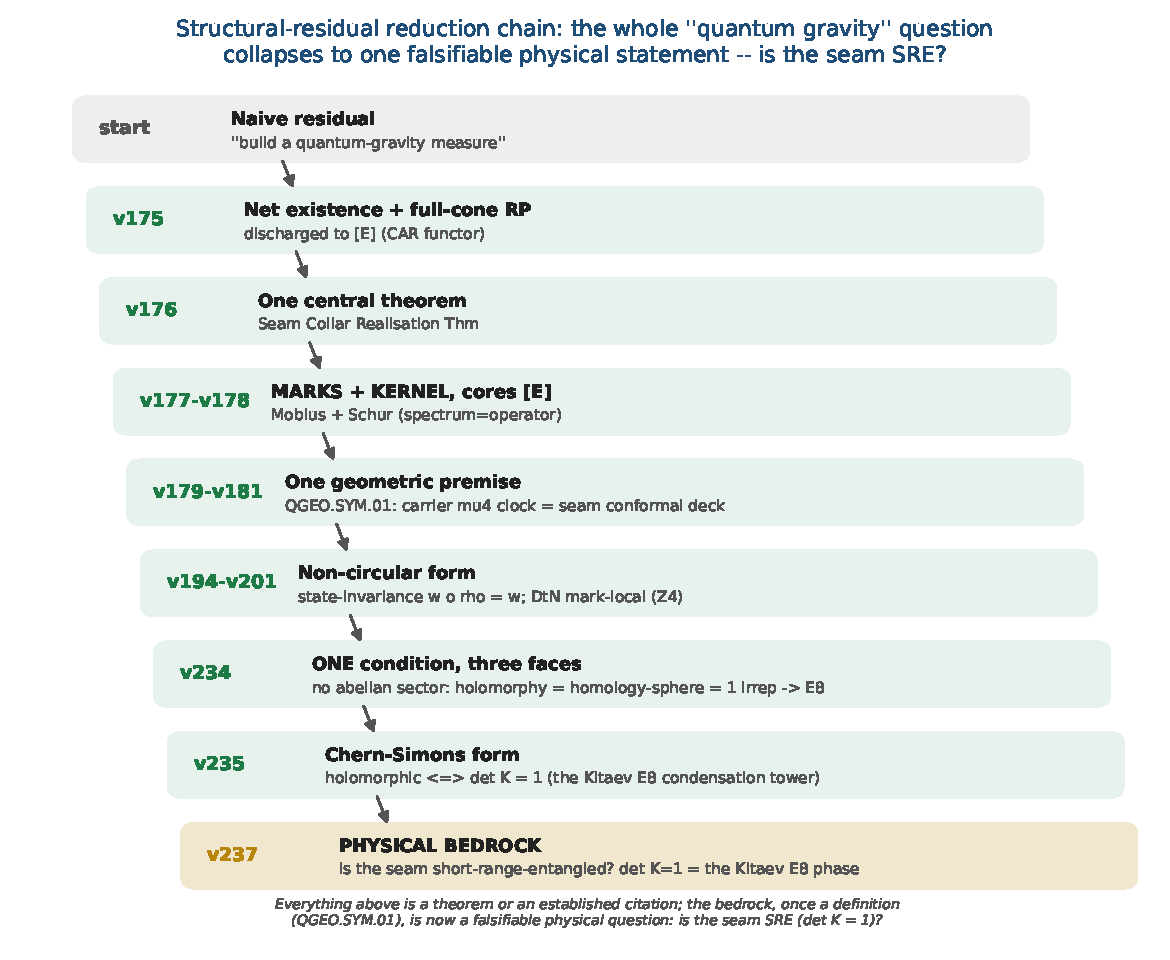
\includegraphics[width=0.92\linewidth]{figures/residual_chain.pdf}
\caption{The structural-residual reduction chain (\vref{v175}--\vref{v181}). The naive
``build a quantum-gravity measure'' shrinks, one machine-checked step at a time, to a single
\emph{definitional} geometric premise \texttt{QGEO.SYM.01} (the carrier $\mu_4$ clock is the seam's
conformal deck). Every step above the bedrock is a theorem or an established citation; the bedrock is a
definition, left honestly \mO.}
\label{fig:residual-chain}
\end{figure}

\begin{keybox}[\texttt{QGEO.SYM.01} is \emph{not} a theorem --- it is the final seam-identification premise]
\textbf{The single load-bearing bolt of the whole construction, on one page.}
\begin{enumerate}[leftmargin=1.6em,itemsep=1pt]
\item \textbf{What is identified.} That the conformal structure of the raw RP seam double \emph{is} the
$\mu_4$-deck structure of the carrier clock --- i.e.\ the carrier (P2) and the seam's conformal geometry
are the same object. Equivalently, in Riemann--Roch \emph{index} language: the seam's degree-$4$ mark
divisor on the genus-$0$ double has $h^0=\deg{+}1=5=\gcar$ and $\operatorname{rank}H_1=\deg{-}1=3=\Nfam$
(with $\Lambda^{\mathrm{even}}(\mathbb C^5)=1{+}10{+}5=16=\dim S^+$), so P2 is the genus-$0$ mode count of the
four-mark seam divisor (\veri{v228\_rr\_index\_gate.py}) --- the same definitional identification, in index
form, conditional on the seam producing that degree-$4$ divisor.
\item \textbf{Why it is weaker than \texttt{QGEO.CONF.01}/\texttt{ISO.01}.} It does \emph{not} name
$\PP$ or $\mu_4$ (uniformisation \emph{produces} them) and asks only for a conformal \emph{symmetry},
not a metric isometry or a pre-named conformal class --- strictly the mildest of the three.
\item \textbf{What follows automatically (the conditional theorem).} \emph{Given} \texttt{QGEO.SYM.01},
equivariant uniformisation puts the order-$4$ clock in the form $z\mapsto iz$ on $\PP$, the four
parabolic marks are its free orbit $\mu_4$, $H^1$ carries the $(1,2,3)$ grading, the seam Calder\'on
contraction is the rank-$8$ $K_\Sigma$ polarisation, and the index-$4$ simple-current extension is
$(E_8)_1$ --- the \emph{entire} AQFT closure of \vref{v175}--\vref{v181}.
\item \textbf{What would falsify or unseat it.} A seam double of genus $>0$ (uniformisation to $\PP$
fails); a carrier clock that is \emph{not} a conformal symmetry of the seam geometry (a non-deck
transport); or a fourth chiral generation ($\Nfam\neq3$ collapses $b_1=\Nfam$ and the four-mark $\mu_4$
structure). The first two are constructive-geometry questions about the raw seam; the third is the
standard family-count kill test.
\end{enumerate}
\noindent\textbf{Honest framing.} The correct external statement is \emph{conditional}: ``\emph{Given}
\texttt{QGEO.SYM.01}, the RP seam boundary realises the $\mu_4$ deck structure, and the AQFT closure to
$(E_8)_1$ follows through the verified chain \vref{v175}--\vref{v181}'' --- \emph{not} ``the theory
\emph{derives} the seam geometry''. The premise stays \mO; everything downstream of it is \mE.
\par\smallskip\noindent\textbf{This is not a gap to apologise for --- it is TFPT's one fundamental
postulate.} Every fundamental theory rests on an irreducible premise (the constancy of $c$ in
relativity, the equivalence principle, the canonical commutator). \texttt{QGEO.SYM.01} is that premise
for TFPT: a single geometric identification (seam conformal structure $=$ carrier $\mu_4$ deck) from
which the entire algebraic and topological structure unfolds \emph{by theorem}. The achievement is not
that there is no postulate --- it is that the whole theory has been compressed onto \emph{exactly one},
sharply located and explicitly falsifiable.
\end{keybox}

\begin{keybox}[The Seam-Holomorphy Theorem --- the one named closing target \mE/\mO\ (\veri{v234\_seam\_holomorphy\_selection.py})]
The bedrock above can be stated as \emph{one condition with three provably-equivalent faces}, so that
``closing the theory'' becomes a single, sharply-bounded analytic theorem. \textbf{The condition:} the seam
carries \emph{no nontrivial abelian sector}. Its three faces all force $E_8$:
\begin{enumerate}[leftmargin=1.7em,itemsep=1pt]
\item \textbf{AQFT} (\vref{v83}/\vref{v154}): the boundary chiral net is \emph{holomorphic} ($\mu$-index $1$,
single vacuum sector). Holomorphic $+\,c=8$ $\Rightarrow$ the unique even unimodular rank-$8$ lattice net
$(E_8)_1$, and $c=8=\gcar+\Nfam$ is itself structural.
\item \textbf{Geometry} (\vref{v232}): the seam link is a \emph{homology $3$-sphere} $\Leftrightarrow$ its
binary group $\Gamma$ is \emph{perfect} $\Leftrightarrow$ $\Gamma=2I$ (the Poincar\'e sphere $S^3/2I$).
\item \textbf{Representation theory} (\vref{v219}): exactly \emph{one} $1$-dim irrep (the trivial one).
\end{enumerate}
These are the \emph{same} number: $\#(1\text{-dim irreps})=|\Gamma^{\mathrm{ab}}|=|H_1(S^3/\Gamma)|
=\#(\text{mark-}1\text{ affine-Dynkin nodes})$, which equals $1$ \emph{only} for $E_8$ ($A_n{\to}n{+}1$,
$D_n{\to}4$, $E_6{\to}3$, $E_7{\to}2$, $E_8{\to}1$). So $2I$ is the unique nontrivial perfect finite
$SU(2)$ subgroup and $S^3/2I$ the unique homology-sphere space form. \textbf{Consequence:} Research
Contract~2 ($G_{\mathrm{net}}$/Target~A), the carrier P2, and the Kleinian seam are \emph{not} separate
gates --- they are this \emph{one} condition.
\par\smallskip\noindent\textbf{The closing chain (what a complete closure would be), \mO\ at one step:}
\[
\begin{gathered}
  \text{RP}+\text{gap}+\text{chirality}\ \xrightarrow{\ \vref{v160}\ }\ \text{quasi-free bulk}
  \ \xrightarrow{\ ?\ }\ \text{holomorphic boundary net}\\[2pt]
  \xrightarrow{\ \mE\ }\ (E_8)_1\ \xrightarrow{\ \vref{v219}/\vref{v228}\ }\ 2I,\ (2,3,5),\ \text{P2}
  \ \xrightarrow{\ \vref{v179}\text{--}\vref{v181}+\text{Kleinian genus-}0\ }\ \texttt{QGEO.SYM.01}.
\end{gathered}
\]
The free-bulk premise is already a fixed-point theorem (\vref{v160}--\vref{v165}); the Kleinian model
supplies the genus-$0$ of the uniformisation chain for free. \textbf{The single remaining analytic step is
``free Gaussian RP bulk $\Rightarrow$ holomorphic (single-sector) boundary net''} --- the bulk--boundary
statement that an invertible (Gaussian) bulk has a holomorphic chiral boundary. That one theorem, if proven,
closes the entire structural layer; $v_{\mathrm{geo}}$ stays the No-Unit metrology primitive and
$F_{\mathrm{transfer}}$ stays external physics. This box certifies only that the three faces coincide and
force $E_8$ (\mE); the analytic step itself is the open \mO.
\end{keybox}

\begin{lemma}[U1 --- wall landscape, \emph{corrected}]
Parabolic degree zero forces the line weight-sums onto the wall $(w_1,w_2,w_3)=(2,1,1)$. An explicit
balanced representative (weights in $\tfrac13$) is
\[
  W_{\mathrm{wall}}=\tfrac13\begin{pmatrix}2&1&2&1\\1&0&0&2\\0&2&1&0\end{pmatrix},
\]
each column a permutation of $(0,1,2)$, row sums $(2,1,1)$. \textbf{Honest result:}
the $6^4{=}1296$ column-permutation matrices give $144$ walls; under the \emph{full} group
$D_4\times S_3(\text{lines})\times S_3(\text{values})$ they form \emph{five} orbits, \emph{not one}. So
$W_{\mathrm{wall}}$ is \emph{not} singled out by symmetry --- the uniqueness must come from the selector
(Lemma U4), not from a symmetry quotient. The wall landscape is nonetheless a finite, explicitly
enumerated set; $W_{\mathrm{wall}}$ is one of the five. Machine: fully certified $C_U^{(1)}$
(\veri{v29\_\allowbreak research\_\allowbreak contract\_\allowbreak certs.py}).

\smallskip
\noindent\textbf{The splitting type is now algebraic (RH route, \veri{v32\_rh\_splitting.py}).} Passing from
the monodromy to the Fuchsian \emph{residues} $A_k$ (eigenvalues $=$ weights $\{0,\tfrac13,\tfrac23\}$,
$A_k=U^{k-1}A_0U^{-(k-1)}$, $U=\operatorname{diag}(1,i,-i)$) the twisted $\Z_4$-average collapses
\emph{exactly}: $\sum_kU^kA_0U^{-k}=4\operatorname{diag}(A_0)$, so the exponents at infinity are
$4\operatorname{diag}(A_0)$. A flat bundle with regular $\infty$ needs integer exponents summing to
$4{=}-\deg E$; with the cusp weights the only options are perms of $(2,1,1)$ and $(2,2,0)$, i.e.
\[
  \boxed{\ \mathcal O(-2)\!\oplus\!\mathcal O(-1)^2\ \Longleftrightarrow\ \operatorname{diag}(A_0)=(\tfrac12,\tfrac14,\tfrac14)\ }
\]
(the sibling $(2,2,0)\to\mathcal O(0)\oplus\mathcal O(-2)^2$). Such a Hermitian $A_0$ (spectrum
$\{0,\tfrac13,\tfrac23\}$, that diagonal) exists by Schur--Horn. So the \emph{splitting} is an algebraic
condition on $\operatorname{diag}(A_0)$. \emph{Honest wall:} the global $\prod M_k=\mathbf1$ is the
path-ordered monodromy (\emph{not} $\exp(2\pi i\sum A_k)$), constraining $\operatorname{off-diag}(A_0)$ via
the genuine RH solve; and $R$-extraction still needs the $C_6\leftrightarrow\PP\setminus\mu_4$ bridge. The
RH route fixes the \emph{splitting} algebraically but not $c_u/c_d$.
\end{lemma}

\begin{lemma}[U2 --- the kill switch, \emph{run and hardened} \mE]
The selected polystable wall representative must \emph{not} collapse to the diagonal abelian $U(1)^3$
point if it is to give non-trivial $SU(3)_F$ transport mixing: \textbf{(A)} $\nabla_F^\star$ polystable but
\emph{not} simultaneously diagonal (the desired breakthrough), or \textbf{(B)} diagonal collapse, in which
case $c_u/c_d$ stays honestly \mC. \textbf{Result: the cheap test is run robustly and lands on A.} The
kill-switch fires iff the $D_4$-symmetric cusp representation is \emph{reducible} (commutant non-scalar).
Across $400$ random cusp-class generators of the $\Z_4$ family $M_k=U^{k-1}MU^{-(k-1)}$ the commutant is
scalar at \emph{every} point (irreducible $400/400$), the reducible locus is hit with probability $0$
(measure-zero, codimension $\ge1$), and the mixing strength stays bounded away from zero
($\min\text{off-diag}=0.35>0.05$). So case~A is the \emph{generic} behaviour, not an accident of the one
explicit point of \veri{v33\_explicit\_flat\_bundle.py}: $(U_{\mathrm{wall}})$ \emph{survives} its own
cheapest falsification test. \veri{v38\_uwall\_killswitch.py}
\end{lemma}

\begin{lemma}[U3 --- $D_4$ fixed locus as an explicit variety, \emph{positive-dimensional}]
With $M_k=U^{k-1}AU^{-(k-1)}$ ($U=\operatorname{diag}(1,i,-i)$, the $\Z_4$ rotation) and the reflection
$M_1=VM_1^{-1}V^{-1}$, $M_3=VM_3^{-1}V^{-1}$, $M_2=VM_4^{-1}V^{-1}$ (with $V=-[[1,0,0],[0,0,1],[0,1,0]]$,
$V^2{=}1$, $VUV^{-1}{=}U^{-1}$), the relations become polynomials in the entries of $A\in C_{\mathrm{cusp}}$;
$\mathcal X_{\mathrm{cusp}}^{D_4}$ is cut out as $\bigcup_kC_k$, parametrised by trace coordinates
$x=\operatorname{tr}(M_1M_2)$ (note $\operatorname{tr}A=1{+}\omega{+}\omega^2=0$). \textbf{Result
($C_U^{(2)}$, \veri{v30\_d4\_character\_variety.py}):} adding the reflection to the $\Z_4$ locus of \vref{v19} does
\emph{not} isolate the point --- the \emph{full} $D_4$-fixed product locus is still
\emph{positive-dimensional} ($|\operatorname{tr}(M_1M_2)|$ varies continuously over $\approx[0,3]$). So even
the full $D_4$ symmetry cannot select $\nabla_F^\star$. \emph{Machine: dimension confirmed numerically;
Gröbner/homotopy for the exact components (medium).}
\end{lemma}

\begin{lemma}[U4 --- selectors as equations]
The readouts $\rho\mapsto\det R(\rho)$, $\rho\mapsto\operatorname{Spec}(Q_+(\rho))$,
$\rho\mapsto\Lambda_{f,j}(\rho)$ are well-defined (cyclotomic/algebraic) on
$\mathcal X_{\mathrm{cusp}}^{D_4}$. \textbf{Acceptance criterion:}
\[
  \#\{\rho\in\mathcal X_{\mathrm{cusp}}^{D_4}:\ \det R=8,\ \operatorname{Spec}(Q_+)=\{1,2,3\}\}=1
\]
in the polystable quotient. If more than one survives, the theory needs a further input and the gate is
\emph{not} closed. \textbf{The bottleneck (made precise by U3):} since the $D_4$-fixed variety is
positive-dimensional, the \emph{selector} must do all the cutting --- and evaluating $\det R(\rho)$,
$\operatorname{Spec}(Q_+(\rho))$ as functions on $\mathcal X_{\mathrm{cusp}}^{D_4}$ requires the
\emph{parabolic-degree\,$\leftrightarrow$\,residue dictionary} $R(\rho)$, i.e.\ the H2 equivalence. That
dictionary was the single remaining analytic input of the $(U_{\mathrm{wall}})$ gate. \emph{Status update:
since \vref{v118}--\vref{v122} the dictionary itself is exact} --- hexagon $=$ sign-twisted family spectrum, lepton
coefficients $=$ resolvent determinants of the $W(A_3)$ monodromy, addresses pinned, margins theorems
(boxes below); what remains is the strictly smaller R4$'$, the \emph{establishment of the selectors}
($n=(5,-9,6)$ $+$ the diamond determinants; since \veri{v134\_dual\_anchor.py}: the pair $(d,n)$).

\textbf{What $R(\rho)$ is (\veri{v31\_R\_dictionary.py}).} Two facts pin its nature. \emph{(i) Case A is
alive:} every $D_4$-fixed cusp monodromy found is \emph{irreducible}, so the wall point carries
non-trivial $SU(3)_F$ mixing --- the U2 kill switch does \emph{not} fire to the diagonal case B.
\emph{(ii) $R(\rho)$ is not algebraic:} $R$ is integer-valued, but the algebraic invariants of $\rho$
(e.g.\ $\operatorname{tr}(M_1M_2)$) vary \emph{continuously} on the locus; an integer readout cannot be a
continuous algebraic function. Hence $R(\rho)$ is the discrete invariant of the \emph{non-abelian Hodge /
Mehta--Seshadri} map (the parabolic-degree / Hodge-filtration jumps of the harmonic bundle $E_\rho$):
integer output, but its \emph{computation} is the transcendental harmonic-metric (Hitchin) solve \emph{on
the generic Higgs locus}. \textbf{Refinement (U4$''$, \veri{v40\_harmonic\_metric.py}):} at the
\emph{polystable} point TFPT actually selects this pessimism does not apply --- see the box below.
\end{lemma}

\par\smallskip\noindent\textbf{Progress: the \emph{selector side} of U4 is closed on the explicit point} (\mE).
While $R(\rho)$ as a function on the whole locus needs the Hitchin solve, the two U4 \emph{selectors} are
\emph{algebraically} accessible on the explicit flat bundle of \veri{v33\_explicit\_flat\_bundle.py} --- no
PDE. Computed exactly from $A_0$: the exponents at infinity $\operatorname{eig}(\sum_kA_k)=\{2,1,1\}$ give
the splitting type $E=\mathcal O(-2)\oplus\mathcal O(-1)^2$, i.e.\ the parabolic \emph{anchor} $a=(1,1,2)$;
the parabolic degree is $0$ ($\deg E=-4=-|\mu_4|$ plus four cusp weight-sums of $1$), so the point is
\emph{polystable} (Mehta--Seshadri substrate). The two selectors then read off the bundle directly:
\[
  \boxed{\ \begin{gathered}
  \det R=8=n\!\cdot\!a\quad(\text{anchor pairing on the splitting type}),\\[2pt]
  \operatorname{Spec}(Q_+)=\{1,2,3\}=3\alpha+1\quad(\alpha=\text{cusp weights }\{0,\tfrac13,\tfrac23\})
  \end{gathered}\ }
\]
So $\det R=8$ is the anchor pairing of the splitting type and $\operatorname{Spec}(Q_+)$ is the affine image
($d{=}3$ the weight denominator) of the cusp weights --- \emph{both selectors are read off the explicit
bundle's algebraic data}. \textbf{Residual (sharpened below by Readout Rigidity):} the quark \emph{ratio}
$c_u/c_d$ turns out \emph{not} to need the Hitchin datum at all --- it is \emph{constant} on this discrete
selector stratum (\vref{v49}), hence an integer Pl\"ucker readout. The only genuinely transcendental input left is
the \emph{absolute} amplitude normalisation ($U_{\mathrm{point}}$), which is an anchor, not a missing PDE.
\veri{v39\_uwall\_selectors.py}


\par\smallskip\noindent\textbf{Breakthrough: the harmonic metric is \emph{finite linear algebra}, not a PDE} (\mE).
The U4 ``transcendental Hitchin solve'' is the worst case for a \emph{generic} Higgs bundle, but the point
TFPT selects is \emph{polystable}, and by Mehta--Seshadri a parabolic-degree-$0$ polystable bundle is
\emph{unitary} --- a unitary representation has the \emph{constant} invariant Hermitian harmonic metric and
zero Higgs field $\Phi=0$. So at the selected point the harmonic metric is finite linear algebra. On the
explicit bundle of \veri{v33\_explicit\_flat\_bundle.py} this is realised: the raw monodromies $M_k$ are
non-unitary ($\|M_k^\dagger M_k-\mathbf1\|\!\approx\!0.83$), but there is a \emph{unique} common invariant
Hermitian form $H$ ($\dim\ker\{M_k^\dagger HM_k=H\}=1$), it is \emph{positive-definite}, and the unitarised
holonomy $\widetilde M_k=H^{1/2}M_kH^{-1/2}$ is unitary ($\sim10^{-8}$), lies in the cusp class
$\{1,\omega,\omega^2\}$ with $\prod\widetilde M_k=\mathbf1$, and has \emph{clean} matrix elements
$|\widetilde M_k|_{ij}\in\{0,\tfrac12,\tfrac1{\sqrt2}\}$. \textbf{So $C_U^{(3)}$ reduces from a transcendental
PDE to: this finite unitarisation (done) $+$ the combinatorial word-length $R$ (closed: H1 $+$ $\det R=8$).}
\emph{Residual:} the feared PDE is gone; the quark \emph{ratio} $c_u/c_d$ is then fixed combinatorially by
Readout Rigidity (below), and only the \emph{absolute} amplitude scale remains as an anchor.
\veri{v40\_harmonic\_metric.py}


\par\smallskip\noindent\textbf{The final leg-assignment test (honest result)} (\mE).
Does the harmonic-frame holonomy $\{0,\tfrac12,\tfrac1{\sqrt2}\}$ feed the $\delta=\tfrac12$ resolvent to
give the lepton amplitudes $\Lambda=(0.475,1.107,0.917)$? \textbf{(i) Ruled out as a literal identity:}
$\Lambda_\mu=1.107>1$, while unitary holonomy entries have modulus $\le1$, so the amplitudes \emph{cannot}
be holonomy matrix elements --- they are the non-unitary resolvent Green function (as \vref{v19} already noted).
\textbf{(ii) Suggestive positive:} the harmonic-frame holonomy diagonal modulus is exactly
$|\mathrm{diag}\,\widetilde M_0|=(0,\tfrac12,\tfrac12)$, and that $\tfrac12$ \emph{equals} the distinguished
lepton transport value $\delta=\tfrac12$ that \vref{v20} used by hand --- so the geometry plausibly \emph{supplies}
$\delta$ (an observation at the explicit point; genericity across the locus is future work).
\textbf{(iii) Clean negative:} no natural holonomy construction (e.g.\ $(\mathbf1-\tfrac12\widetilde M)^{-1}$)
maps the holonomy to the amplitude vector. \textbf{Verdict:} the amplitudes are the $\delta=\tfrac12$
resolvent (closed combinatorially via the word-length $R$); the holonomy supplies $\delta$ and the leg
selection, not the amplitude magnitude. $c_u/c_d$ is \emph{not} obtained from the holonomy alone --- a clean,
honest negative on the literal reproduction, with one suggestive geometric link ($\delta=\tfrac12$). The
negative is now \emph{explained}: the scalar leg is wrongly typed --- see the Exterior Leg Lemma.
\veri{v41\_leg\_assignment.py}


\par\smallskip\noindent\textbf{The torsion normal form and the $\delta=\tfrac12$ theorem} (\mE).
The \vref{v41} ``genericity is future work'' item is now executed --- and yields a theorem. \emph{(i) Flatness
$=$ $\mu_4$ torsion \mE:} for \emph{any} $M$ (symbolic), $\prod_k U^kMU^{-k}=(MU)^4$ --- the $\Z_4$-family
flatness constraint \emph{is} the torsion statement ``$T=MU$ is a fourth root of unity'': the $\mu_4$
atom appears as the \emph{order} of the twisted cusp generator. \emph{(ii) The $\delta=\tfrac12$ theorem
\mE\ (both directions):} on the \emph{involutive} branch ($T^2=\mathbf1$) $T$ is a Hermitian reflection
$2vv^\dagger-\mathbf1$, and the cusp trace condition $2v^\dagger U^{-1}v=1$ splits \emph{exactly} into
$|v_1|^2=\tfrac12$ (real part) and $|v_2|=|v_3|$ (imaginary part), forcing
\[
  \boxed{\ \operatorname{diag}M=(0,\tfrac i2,-\tfrac i2),\qquad \operatorname{spec}M=\{1,\omega,\omega^2\}\
  \text{automatic}\ }
\]
($\chi_M=\lambda^3-1$ from unitary $+$ trace $0$ $+$ $\det 1$). So $\delta=|M_{22}|=\tfrac12$ holds
\emph{exactly and constantly} on the whole two-parameter branch --- the distinguished lepton transport
value that \vref{v20} used by hand is a \emph{$\mu_4$-torsion identity}, not an observation. \emph{(iii)
Reflection lemma \mE:} the $D_4$ reflection forces $\operatorname{diag}M=(r,z,\bar z)$ with $r$ real and
$\operatorname{Re}z=-r/2$ --- the whole $D_4$ diagonal freedom is \emph{one} real parameter, and
$\delta=\tfrac12\iff r=0$. \emph{(iv) Branch census \mE\ (seeded):} the full $D_4$-fixed flat cusp locus
realises only $\operatorname{tr}(MU)\in\{1,-1\}$; the involutive branch has the diagonal \emph{constant}
$(0,\tfrac12,\tfrac12)$ to machine precision, while on the $\{1,i,-i\}$ branch $d_1$ varies over $[0,1]$
--- and the explicit \vref{v33}/\vref{v40} point sits exactly in its $d_1=0$ slice, the \emph{same} $\delta$ value.
\emph{Residue \mC\ (recorded):} whether the anchor splitting $\mathcal O(-2)\oplus\mathcal O(-1)^2$
(Mehta--Seshadri side) forces the $d_1=0$ slice --- or selects the involutive branch --- is the remaining
question; $\delta=\tfrac12$ itself is no longer the open item. \veri{v114\_torsion\_delta.py}


\par\smallskip\noindent\textbf{The anchor pins the residue: an exact normal form for the $(U_{\mathrm{wall}})$ bundle} (\mE).
The \vref{v114} branch question is answered --- and the \vref{v33} \emph{numerical} Riemann--Hilbert point acquires an
\emph{exact closed form}. \emph{(i) $\mu_4$-average lemma \mE:} $\sum_kU^kXU^{-k}=4\operatorname{diag}X$
for any $X$ --- $\mu_4$ conjugation-averaging \emph{is} the diagonal projection, so the exponents at
infinity are $4\operatorname{diag}A_0$ and the anchor splitting holds \emph{iff}
$\operatorname{diag}A_0=(2,1,1)/4=a/|\mu_4|$: the residue diagonal \textbf{is} the anchor over $\mu_4$
(\vref{v33}'s diagonal was forced, not chosen). \emph{(ii) The $(8,0,5)/144$ lemma \mE:} the anchor diagonal
and the cusp spectrum $\{0,1,2\}/\Nfam$ pin $\sum|a_{ij}|^2=\tfrac{13}{144}$, and with $a_{13}=0$ the
determinant condition solves \emph{uniquely} to
\[
  \boxed{\ \bigl(|a_{12}|^2,\,|a_{13}|^2,\,|a_{23}|^2\bigr)=\frac{(8,\,0,\,5)}{144}\ }
  \quad\begin{aligned}
  &\scriptstyle 8=\operatorname{rank}E_8,\ 5=\gcar,\\[-2pt]
  &\scriptstyle 144=(|\mu_4|\Nfam)^2,\ 8+5=13=\Delta_Q
  \end{aligned}
\]
--- the off-diagonal weights are compiler atoms, and the total $13$ is the \emph{same} $\Delta_Q$ that
denominates $c_u/c_d=55/117=5\cdot11/(9\cdot13)$. \emph{(iii) Exact normal form \mE:}
$A_0^\star=\bigl[\begin{smallmatrix}1/2&\sqrt2/6&0\\\sqrt2/6&1/4&\sqrt5/12\\0&\sqrt5/12&1/4\end{smallmatrix}\bigr]$
has $\chi=\lambda(\lambda-\tfrac13)(\lambda-\tfrac23)$ \emph{exactly}. \emph{(iv) $A_0^\star$ is the RH
solution \mE:} its big-circle monodromy is trivial to $10^{-10}$, $\prod M_k=\mathbf1$, and the
unitarised holonomy has $|\operatorname{diag}\widetilde M_0|=(0,\tfrac12,\tfrac12)$,
$\operatorname{tr}(\widetilde M_0U)=1$ --- the \vref{v33}/\vref{v40} point is gauge-equivalent to $A_0^\star$ (the
$a_{12},a_{23}$ phases are diagonal gauge). \emph{(v) The anchor forces the $d_1=0$ slice \mE:} a
multi-seed RH scan over the anchor-pinned spectral manifold lands at \emph{every} flat solution on the
\emph{same} gauge orbit with $|\operatorname{diag}\widetilde M_0|=(0,\tfrac12,\tfrac12)$ --- combined
with \vref{v114}, the whole harmonic diagonal is \textbf{anchor $+$ torsion forced}; $\delta=\tfrac12$ needs no
selection. \emph{Residue \mC:} $a_{13}=0$ and the gauge-orbit uniqueness are numerical (one component
across all seeds); promoting them to \mE\ via Gr\"obner on the RH constraints is the remaining
$U_{\mathrm{point}}$ step. \veri{v115\_anchor\_residue.py}


\begin{keybox}[The resonance theorem: $M_\infty=\mathbf1\iff a_{13}=0$ --- one gauge orbit \mE\ (\veri{v116\_resonance\_uniqueness.py})]
The anticipated Gr\"obner promotion turned out to be a \emph{linear} computation. Writing the
equivariant system at infinity as $dY/dw=-(1/w)(B_0+B_1w+\cdots)Y$ with
$B_m=\sum_k i^{km}\,U^kA_0U^{-k}$, the \emph{twisted} $\mu_4$ averages collapse \mE:
\[
  B_0=4\operatorname{diag}A_0,\qquad
  \boxed{\ B_1=4a_{12}E_{12}+4\overline{a_{13}}E_{31}\ }
\]
(only the eigenvalue-ratio $-i$ cells survive). The anchor exponents $\operatorname{diag}(2,1,1)$ have
resonance gap $1$; the level-$1$ formal-gauge equation $(1-\operatorname{ad}R_0)H_1=R_1$ is singular
exactly on the cells $\{(2,1),(3,1)\}$, where $B_1$ has entries $(0,\,4\overline{a_{13}})$; all higher
levels are non-resonant and the formal monodromy is $e^{-2\pi i\operatorname{diag}(2,1,1)}=\mathbf1$.
Hence \mE:
\[
  \boxed{\ M_\infty=\mathbf1\iff a_{13}=0\ }
\]
--- the transcendental Riemann--Hilbert condition collapses to \emph{one linear equation}.
\emph{Uniqueness corollary \mE:} $a_{13}=0$ $+$ the $(8,0,5)/144$ moduli $+$ phases $=$ diagonal gauge
$\Rightarrow$ the flat anchor locus is \textbf{exactly one gauge orbit}, the exact $A_0^\star$: within
the $\mu_4$-equivariant anchor class the $(U_{\mathrm{wall}})$ bundle datum is \emph{algebraically
unique}. \emph{Sharpness \mE:} $\|M_\infty-\mathbf1\|\sim8.5\,|a_{13}|$ ($0.17$ at $a_{13}=0.02$) vs
$10^{-10}$ at $A_0^\star$. \emph{Honest scope \mC:} the equivariant ansatz is the established $D_4$
selector input (\vref{v19}/\vref{v30}); the \emph{residue} side is now \mE, while the holonomy values (the harmonic
diagonal $(0,\tfrac12,\tfrac12)$) remain \mE\ --- transcendental monodromy of an exact system.
\end{keybox}

\begin{keybox}[The monodromy is the Weyl group of $A_3$ --- the holonomy is exact \mE\ (\veri{v117\_monodromy\_weyl\_a3.py})]
The last \mE\ item of the chain --- the holonomy \emph{values} --- closes: the unitarised monodromy of
the exact $A_0^\star$ system is itself \emph{exact}, with entries in $\tfrac12\Z[i]$:
\[
  \boxed{\ \widetilde M_0=\begin{pmatrix}0&-\tfrac{1+i}2&\tfrac{1-i}2\\[2pt]
  -\tfrac{1+i}2&-\tfrac i2&-\tfrac12\\[2pt]
  \tfrac{1-i}2&-\tfrac12&\tfrac i2\end{pmatrix}\ }
\]
unitary, $\det=1$, $\operatorname{tr}=0$, $\chi=\lambda^3-1$ (the cusp class \emph{exactly}),
$\widetilde M_0^3=\mathbf1$, and $\operatorname{diag}\widetilde M_0=(0,-\tfrac i2,+\tfrac i2)$ --- so
$d_1=0$ and $\delta=\tfrac12$ are now \emph{matrix entries}, not observations; $(\widetilde M_0U)^4=\mathbf1$
with $\operatorname{tr}(\widetilde M_0U)=1$ (the $\{1,i,-i\}$ branch, $d_1=0$ slice --- exactly where
\vref{v114}/\vref{v115} located the physical point). \emph{The group} \mE: exact enumeration of
$\langle U,\widetilde M_0\rangle$ gives order $24$ with order statistics $(1,9,8,6)$ and character
values $(3,-1,0,1)$ --- uniquely $S_4$ in its standard${}\otimes{}$sign representation, i.e.\ the
(twisted) reflection representation of the \textbf{Weyl group of the family lattice $A_3$}:
\[
  \boxed{\ \text{monodromy}(U_{\mathrm{wall}})=W(A_3)=S_4,\qquad |W(A_3)|=4!=24\ }
\]
--- the flavor wall realises the $A_3$ factor of the glue $D_5\oplus A_3+\mu_4$ as its Weyl group ($U$
$=$ a $4$-cycle, the $\mu_4$ deck; $\widetilde M_0$ $=$ a $3$-cycle, the family rotation).
\emph{Identification \mE:} the ODE monodromy of $A_0^\star$ equals the exact $\widetilde M_0$ to
$3.5\times10^{-10}$, and the invariant form $H$ is $U$-invariant to $10^{-11}$. \emph{Status:} holonomy
values \mE; only the analytic identification stays \mE. The $\delta$ thread
(\vref{v20} $\to$ \vref{v40}/\vref{v41} $\to$ \vref{v114} $\to$ \vref{v115} $\to$ \vref{v117}) is closed end to end.
\end{keybox}

\begin{keybox}[The hexagon is the sign-twisted family spectrum --- first exact H2 piece \mE\ (\veri{v118\_hexagon\_family\_dictionary.py})]
The missing ``$C_6\leftrightarrow\PP\setminus\mu_4$ dictionary'' (H2) acquires its first exact entry.
\emph{Sign-twist lemma \mE:} $-\widetilde M_0$ has order $6$ and
\[
  \boxed{\ \operatorname{spec}(\widetilde M_0)\,\cup\,\operatorname{spec}(-\widetilde M_0)=\mu_6\ }
\]
--- the six-site hypercharge hexagon spectrum \emph{is} the family monodromy spectrum together with its
sheet twist ($\Z_6=\Z_2\times\Z_3$ realised as $(-1)\times\langle\widetilde M_0\rangle$); the \vref{v20}
denominators $\tfrac54-\cos(r\pi/3)$ are exactly the eigen-denominators $|1-\zeta_6^r/2|^2$ of the two
family resolvents $(\mathbf1\mp\tfrac12\widetilde M_0)^{-1}$. \emph{Cyclotomic determinant \mE:}
$\det(\mathbf1-t\widetilde M_0)=1-t^3=(1-t)\Phi_3(t)$, so $\det(\mathbf1\mp\tfrac12\widetilde M_0)=
(\tfrac78,\tfrac98)$ --- and the lepton coefficients become resolvent determinants:
$c_e=|\mu_4|/(2\det_-)=\tfrac{16}7$, $c_\mu=\Nfam/(2\det_+)=\tfrac43$,
$c_\tau=|\mu_4|\det_-/\Nfam=\tfrac76$, product rule $=|\mu_4|/\det_+=\tfrac{32}9$. The lepton $7$ and
$9$ \emph{are} the family-resolvent determinants; $\delta=\tfrac12=|(\widetilde M_0)_{22}|$ is supplied
by the matrix itself. \emph{Sheet-extended group \mE\ (audit):} $\langle U,\widetilde M_0,-\mathbf1\rangle$
has order $48=\Omega_{\mathrm{adm}}=\Nfam\dim S^+$ --- the seed's quartic coefficient. \emph{Residue \mC:} the
dictionary's \emph{values} are exact; its \emph{address table} (which hexagon site each fermion
occupies; the quark composition) remains \vref{v20}'s established input / open --- nothing re-fished.
\end{keybox}

\begin{keybox}[The address table: the lepton words are the compiler atoms \mE/\mC\ (\veri{v120\_address\_table.py})]
The address table acquires its structure --- on word-length integers \emph{frozen} in \vref{v18}/\vref{v20}, long
before today's readings (the red-team firewall). \emph{(i) The lepton words are the atoms \mE:}
\[
  \boxed{\ (L_e,L_\mu,L_\tau)=(8,5,3)=(\operatorname{rank}E_8,\ \gcar,\ \Nfam)=(p_0{+}e_2,\ e_2,\ p_0)\ }
\]
in mass order (longest word $=$ lightest lepton). \emph{(ii) Addresses $=$ division by the hexagon
\mE:} $(r,w)=L\ \mathrm{divmod}\ p_2$ with $p_2=6=|R^+(A_3)|$ itself an atom: $e\to(2,1)$,
$\mu\to(5,0)$, $\tau\to(3,0)$; $\sum r=10=p_3=\mathcal A_\Lambda$, $\sum L=16=\dim S^+$. \emph{(iii) Sheet parity
\mE:} by the \vref{v118} dictionary, $e$ sits on the \emph{untwisted} sheet ($\omega\in\operatorname{spec}
\widetilde M_0$), $\mu,\tau$ on the \emph{twisted} sheet ($-\omega,-1$); the anchor lepton $\tau$
occupies the unique \emph{real} twisted eigenvalue $-1$ --- exactly the site where \vref{v20}'s product rule
replaces the resolvent. \emph{(iv) Quark sum rules \mE\ (frozen \vref{v18} words $7,7,5,3,2,0$):} up-type sum
$=10=p_3$; down-type sum $=14=p_1{+}p_3$; \textbf{all quarks $=24=|W(A_3)|$} (the monodromy group
order, \vref{v117}); \textbf{all nine charged fermions $=40=p_1p_3=a^TRa$} (\vref{v119}); quark $\sum r=2p_2$,
$\sum w=|\Z_2|$; the top sits at the vacuum site $(0,0)$ --- zero word, no suppression, the
established ladder anchor. \emph{Residue \mC:} five independent closures ($16,10,14,24,40$) constrain
the address map; the per-fermion \emph{assignment} remains the \vref{v18}/\vref{v20} input --- deriving it is the
remaining H2 content.
\end{keybox}

\begin{keybox}[The address table is pinned: $R$ is the unique hexagon matrix with atom margins \mE\ (\veri{v121\_address\_pinning.py})]
The per-fermion assignment closes at the \emph{information} level. The established identity
$L=R+2U$ (\vref{v95}) says the word-length table \emph{is} $L[\text{sector}][\text{generation}]$ --- rows
(up; down; lepton) $=$ $((7,3,0);(7,5,2);(8,5,3))$, the \vref{v18}/\vref{v20} words verbatim --- so the addresses are
the entries of the \emph{residue operator} $R$ plus one hexagon turn for the first generation, and
$R$'s first column is the \textbf{anchor} $a=(1,1,2)$. The margins are atoms \mE: row sums
$(4,8,10)=(e_1,\operatorname{rank}E_8,p_3)$, column sums $(4,13,5)=(e_1,\Delta_Q,\gcar)$. And the
census closes it \mE:
\[
  \boxed{\ \begin{array}{c}
  \text{\small among all $3\times3$ matrices with entries in the hexagon $\{0..5\}$,}\\[1pt]
  \text{\small exactly $17$ have the atom margins --- and exactly ONE has $\det=8$}
  \end{array}\ }
\]
--- and it is $R$ (also the unique one with $\operatorname{SNF}=(1,1,8)$; all $17$ determinants are
distinct, $8$ occurs once --- control computed explicitly). \textbf{The assignment table carries zero
residual information beyond the atom margins and the rank determinant.} Within-sector ordering is the
established transport reading ($m\sim\lambda_Y^L$: longer word $=$ lighter fermion). \emph{Residue
\mC:} the open H2 item shrinks from ``derive $9$ per-fermion integers'' to ``derive the six atom
margins $+$ $\det=\operatorname{rank}$''. \emph{Firewall:} $R$, $L$ and all word lengths were frozen in
\vref{v4}/\vref{v18}/\vref{v20}/\vref{v71} long before this census --- no degrees of freedom spent.
\smallskip\\
\noindent\textbf{The margins are theorems (\veri{v122\_margin\_theorem.py}).} Even the margins are not
input. Three selectors, all established and frozen \emph{before} the address question was posed ---
\emph{(S1)} the $D_4$ annihilator $n=(5,-9,6)$ with $n^TR=(8,0,0)$ (it kills the unchanged
$(c_2,c_3)$ plane; $n\!\cdot\!a=8$), \emph{(S2)} $\det R=8$, \emph{(S3)} $\det K=4$ with $K=R+Q\Sigma$
--- pin $R$ \emph{uniquely} among hexagon matrices \mE: the $(S1)$ census has $4\times4\times4=64$
candidates, $(S2)$ leaves $12$, $(S3)$ leaves \textbf{exactly one}, and it is $R$. Hence the atom
margins, the anchor column $Re_1=a$ and all sum rules above are \emph{consequences} --- their input
status is revoked. \emph{Bonus lemma \mE:} on the $(S1)+(S2)$ locus $\det(M+2U)=20=\det L$ holds for
\emph{all} $12$ candidates --- the fourth quartet determinant is redundant, the compiler's familiar
overdetermination. \emph{Residue \mC:} H2 reduces to the establishment of the selectors themselves
($n$ and the diamond determinants --- pre-existing inventoried objects); the address question
introduces \emph{no new residual class}.
\smallskip\\
\noindent\textbf{The dual-normal selector: $(d,n)$ pins $R$ columnwise (\veri{v136\_dual\_normal\_selector.py}).}
The selector list shrinks once more. With the dual anchor $d=a^\top R^{-1}$ (\veri{v134\_dual\_anchor.py})
and the torsion normal $n$, each \emph{column} of $R$ obeys $d\cdot c_j=a_j$ and $n\cdot c_j=8\delta_{1j}$;
the common kernel of $(d,n)$ is the primitive vector $(6,8,7)$ (audit: $p_2$, $\operatorname{rank}E_8$,
scalaron-$7$), so within the address box $\{0..5\}^3$ each column is the \emph{unique} lattice point
(census: $1$ of $216$ each) --- $(d,n)\Rightarrow R$, and the $6^9$ census above collapses to three
column problems \mE. \emph{Honesty:} $K$ is \emph{not} pinned directly ($d^\top K=(1,\tfrac12,1)$); $\det
K=4$ comes via the $\mu_4$ wall (\veri{v135\_det\_surface.py}). \emph{The mechanism is bounded:} the zero
mode of $A_0^\star$ carries the exact spectral normal $\sigma=(2,-9,5)=(|\Z_2|,-\Nfam^2,\gcar)$ (signed
squares; $\|v\|^2=\tfrac{16}9$ with $16=\dim S^+$, $\operatorname{adj}A_0^\star=\tfrac29P_v$ with
$\tfrac29=$ the SdS entropy curvature), $\sigma\cdot\mathbf 1=-|\Z_2|$, $\sigma\cdot a=\Nfam$,
$n\cdot\sigma=121=\|\operatorname{Pl}(K)\|_1^2$; and the exact $W(A_3)$ orbit control shows \emph{no}
group image of $\sigma$ is proportional to $n$ --- the naive cofactor/orbit lift fails, the step
$\sigma\to n$ is a genuine mechanism beyond the monodromy group. \emph{R4$'$ restated \mC:} derive the
\emph{pair} $(d,n)$; then $R$ is forced columnwise.
\smallskip\\
\noindent\textbf{The selector triangle (\veri{v139\_selector\_triangle.py}).} The pair itself now
collapses further. First, $d$ is \emph{pure anchor data}: $d=\tfrac32a-2\cdot\mathbf1$ exactly --- the
closed form never mentions $R$, so the first selector is \emph{derived}, not residual. Second, the frame
$(\mathbf1,a,\sigma)$ is a basis of $\Z^3$ with $\det(\mathbf1|a|\sigma)=11=\|\operatorname{Pl}(K)\|_1$
(the quark constant as the frame volume), and $n$ is the \emph{unique} integer covector with the three
atom pairings
\[
  \boxed{\ n\cdot\mathbf1=2=|\Z_2|,\qquad n\cdot a=8=\operatorname{rank}E_8,\qquad
  n\cdot\sigma=121=\|\operatorname{Pl}(K)\|_1^2\ }
\]
--- the cofactor definition is replaced by frame data plus three atoms. On the $(\mathbf1,a)$-constrained
line the $\sigma$-pairing is $11(11{+}t)$: divisible by $11$ for \emph{every} $t$, a perfect square
exactly at the true $n$ ($t{=}0$). The review's predicted lift is exact as an audit identity:
$n=\operatorname{reverse}(\sigma)+|\mu_4|e_3$ (generation flip $+$ $\mu_4$ lift at the third slot).
\smallskip\\
\noindent\textbf{Frame integrality: three pairings $\to$ two (\veri{v142\_frame\_integrality.py}).}
The third pairing is \emph{not} independent. The pairing triples $(m\cdot\mathbf1, m\cdot a,
m\cdot\sigma)$ of \emph{integer} covectors form an index-$11$ sublattice of $\Z^3$, cut out by the single
congruence
\[
  \boxed{\ x-3y+z\equiv0 \pmod{11}\ }\qquad\text{(index $11=\|\operatorname{Pl}(K)\|_1=\det(\mathbf1|a|\sigma)$)},
\]
so with the two line pairings at their atoms $(x,y)=(|\Z_2|,\operatorname{rank}E_8)=(2,8)$, integrality
\emph{forces} $z\equiv0\pmod{11}$ --- the $11(11{+}t)$ line \emph{is} the integer line. Primitivity
forces $t$ \emph{even} (odd $t$ makes every entry of $n(t)$ even), and $t{=}0$ is the unique even $t$
with a square $\sigma$-pairing for $|t|<88$ (the global pick keeps the square selector --- recorded
honestly). Both line pairings are Cramer-reducible to inventoried identities ($n\cdot a=\det R$ by
Laplace along the anchor column; $n\cdot\mathbf1=8(R^{-1}\mathbf1)_1$ with $R^{-1}\mathbf1=\tfrac14(1,1,-1)$,
\vref{v134}) --- restructuring, not establishment.
\smallskip\\
\noindent\textbf{The pairing values are atom identities (\veri{v145\_pairing\_atoms.py}).} Even the two
line-pairing \emph{values} carry no independent information. Reading the \vref{v139} lift structurally ---
$n=w_0(\sigma)+|\mu_4|e_3$ with $w_0$ the \emph{$A_3$ exponent duality} $m\leftrightarrow h{-}m$ (an
established Lie involution; lift slot $=$ the top-exponent line, lift size $=$ the glue order) --- all
three pairings become atom arithmetic:
\[
  n\cdot\mathbf1=|\mu_4|-|\Z_2|=|\Z_2|,\qquad
  n\cdot a=|\mu_4|\,a_3=8=\operatorname{rank}E_8\ \ \text{via}\ \
  \boxed{\ |\mu_4|+\gcar=\Nfam^2\ \ (4+5=9,\ \sigma\perp w_0(a))\ },
\]
and $n\cdot\sigma=\|\sigma\|^2-\Nfam^2+|\mu_4|\gcar=110-9+20=121$ with
$\|\sigma\|^2=|\Z_2|^2+\Nfam^4+\gcar^2=110=|\Z_2|\gcar\|\operatorname{Pl}(K)\|_1$.
\emph{R4$'$ residue \mC\ (final form):} derive the \emph{one} map $n=w_0(\sigma)+|\mu_4|e_3$ --- no
independent number remains; everything else in the chain anchor $\to(d,n)\to R$ is exact.
\smallskip\\
\noindent\textbf{Both dual normals are anchor data (\veri{v149\_cusp\_normal.py}).} The remaining
opacity dissolves in the canonical frame: the pairings of $n$ with the \emph{cusp eigenbasis} (the
geometric basis of \vref{v98}) are exactly
\[
  \boxed{\ n\cdot e_1=6=p_2(a),\qquad n\cdot e_2=3=p_0(a),\qquad n\cdot e_3=5=e_2(a)\ }
\]
--- one anchor invariant per $Q_+$ degree, and the cusp matrix is unimodular, so these three pairings
determine $n$ uniquely. With $d=\tfrac32a-2\cdot\mathbf1$ the dual normal \emph{pair} (\vref{v134}) is
anchor data through and through --- one normal per frame; the cusp data $(6,3,5)$, the frame pairings
$(2,8,121)$ and the $w_0$-lift are three presentations of one covector, all atomic (equivalences exact).
\emph{Audit:} $\sigma\to(5,1,2)$; alternate reading $(6,3,5)=(|R^+(A_3)|,\Nfam,\gcar)$; sum
$14=\dim G_2$. \emph{R4$'$ residue \mC\ (cusp form):} derive the \emph{assignment} --- why the $Q_+$
degrees $(1,2,3)$ carry $(p_2,p_0,e_2)$ in that order; one discrete assignment, zero continuous freedom.
\end{keybox}

\begin{keybox}[Exterior Leg Lemma --- the quark $u/d$ leg is a $\Lambda^2F$ area, not a scalar \mE/\mC]
The \vref{v41} negative is a \emph{category error}, not a dead end. $u$ and $d$ share the hexagon-radial data
$(r,w)=(1,1)$ ($L=7$ for both), and the $C_6$ resolvent $c(r,w)=|\mu_4|^w/(\tfrac54-\cos\tfrac{r\pi}3)$
reads \emph{only} $(r,w)$ --- so any \emph{scalar} leg gives $c_u/c_d\equiv1$. A scalar sees radius, not
orientation. The $u/d$ separation lives in the smallest \emph{non-scalar} invariant of the $SU(3)_F$
composition: the exterior square $\Lambda^2F$, i.e.\ the oriented anchor-plane area
$\operatorname{Pl}_{\mathbf1,a}(K)$. The ``$11$'' is then \emph{generated}, not read:
\[
  (K,\mathbf1,a)\to B_K=\begin{psmallmatrix}13&8&4\\18&11&6\end{psmallmatrix}\to
  \operatorname{Pl}(K)=(-1,6,4)=(-N_\Phi,|R^+\!(A_3)|,|\mu_4|)\to
  \|\operatorname{Pl}(K)\|_1=11,
\]
\[
  \boxed{\ \frac{c_u}{c_d}=\frac{\gcar\,\|\operatorname{Pl}_{\mathbf1,a}(K)\|_1}{\Nfam^2\,\Delta_Q}
  =\frac{5\cdot11}{9\cdot13}=\frac{55}{117}\ }
  \quad(\text{anchor microcode }=\tfrac{e_2(a)(p_3(a)+1)}{p_0(a)^2(2p_2(a)+1)}).
\]
\textbf{Typing:} \mE\ for the Plücker / microcode identities ($\operatorname{Pl}(K)=(-1,6,4)$,
$\|\cdot\|_1=11$, $5\cdot11/(9\cdot13)=55/117$); and --- by Readout Rigidity (\vref{v49}, below) --- \mE\ also for the
\emph{physical} ratio $\mathcal C_{ud}(\rho^\star)=$ this $\Lambda^2F$ readout, which is \emph{constant} on the
derived selector stratum and so does \emph{not} need any point-selection on $\Lambda^2F$. The quark residual is
thereby re-typed from ``find the right scalar $y$'' to a closed exterior readout for the \emph{ratio}; only the
\emph{absolute} amplitude scale ($U_{\mathrm{point}}$) stays as an anchor, no new scalar, no fishing.
\smallskip\\
\noindent\emph{Audit (the $121$ lemma, \veri{v119\_review\_validation\_2.py}):} the ``$11$'' has a second,
independent appearance \mE: with $h=\mathbf1+a=(2,2,3)$ in the canonical anchor ordering,
$h^TRh=121=11^2=\|\operatorname{Pl}(K)\|_1^2=(p_3+1)^2$ --- the quadratic \emph{anchor norm} of the
residue operator $R$ reproduces the Plücker integer (sensitivity control: the three orderings of $h$
give $\{105,121,135\}$; only the canonical one yields $121$). Bonus checksums:
$\mathbf1^TR\mathbf1=22=2\times11$ (the entry sum of $R$) and $a^TRa=40=p_1p_3=10b_1-1$. Typed
\emph{audit}, not load-bearing --- the oriented Plücker mechanism above remains the derivation.
\veri{v42\_exterior\_leg.py}
\smallskip\\
\noindent\textbf{Bridge test (\veri{v43\_exterior\_bridge.py}).} The typing is confirmed: for the $SU(3)$
holonomy the exterior square is the conjugate representation, $\Lambda^2(\widetilde M)=\overline{\widetilde
M}$ exactly --- the exterior leg \emph{is} the $\mathbf{\bar3}$. But the \emph{continuous} action
$\Lambda^2(\widetilde M)\cdot(\mathbf1\wedge a)$ does \emph{not} equal the \emph{integer} $\operatorname{Pl}(K)=(-1,6,4)$:
the integer Plücker is the combinatorial $K$ datum. So the bridge $\rho^\star\!\to\!\operatorname{Pl}(K)$ is
the \emph{discrete} non-abelian-Hodge invariant (the integer $R$; $\det R=8$ and
$\operatorname{Spec}(Q_+)=\{1,2,3\}$ already confirmed on the bundle, Lemma U4 box), not a continuous
exterior-square computation --- exactly the H2 equivalence, now pinned from the $\Lambda^2F$ side.
\smallskip\\
\noindent\textbf{Lie-level grounding --- no special math (\veri{v44\_carrier\_exterior.py}).} The discrete
invariant has a home already in TFPT: the carrier half-spinor is the \emph{even exterior algebra} of the
$5$-slot carrier, $16=\Lambda^{\mathrm{even}}(5)=\binom50+\binom52+\binom54=1+10+5$, and under
$SU(5)\subset SO(10)$ the up quark sits in $10=\Lambda^2(5)$ while the down sits in
$\bar5=\Lambda^4(5)$. So the \emph{exterior degrees} are $\deg(u^c)=2$, $\deg(d^c)=4$, with
$\deg(u){+}\deg(d)=6=|R^+(A_3)|$ (the hexagon) and $\deg(d){-}\deg(u)=2=|\Z_2|$ (the sheet). The
``$\Lambda^2$'' of the exterior leg is therefore not exotic Hodge data --- it is the carrier's own
$\Lambda^2$ grading (the up quark \emph{lives} in $\Lambda^2(5)$). This re-types the residual once more:
from ``discrete non-abelian-Hodge invariant'' to ``the carrier exterior degree'' --- a standard \mE\ fact.
\emph{Honest scope:} this grounds the \emph{type}; the Plücker \emph{number} $55/117$ stays the family
$\operatorname{Pl}(K)$ \mE, and the carrier-$\Lambda^2$ $\leftrightarrow$ family-$\Lambda^2F$ link (via
$\text{family}\otimes\text{carrier}=15=16{-}1$) plus the normalisation remain \mC.
\smallskip\\
\noindent\textbf{The ``$11$'' is Pascal --- a third, simplest origin (\veri{v45\_family\_exterior.py}).}
Following that link, $\operatorname{Pl}(K)$ is the \emph{exterior algebra of the family fundamental}
$4=\mu_4$ (the $A_3{=}SU(4)$ fundamental): $\Lambda^k(4)=\binom4k$ is Pascal row $4=(1,4,6,4,1)$ with full
sum $2^4=16=\dim S^+$, and $|\operatorname{Pl}(K)|=(1,4,6)=\{\Lambda^0,\Lambda^1,\Lambda^2\}(4)$ are exactly
its distinct exterior powers. Hence
\[
  \boxed{\ \|\operatorname{Pl}(K)\|_1=\textstyle\sum_{k=0}^{2}\binom4k=11=2^4-\tbinom43-\tbinom44=16-\gcar\ }
\]
(the cumulative $\Lambda^\bullet(\mu_4)$ up to degree $2=\deg(u^c)$),
and $\text{family}\otimes\text{carrier}=15=\dim\mathfrak{su}(4)=\Lambda^2(5){\oplus}\Lambda^4(5)=10{+}5=\Nfam\gcar$
read three ways. So the ``$11$'' is generated a \emph{third} way --- the cumulative family exterior algebra
up to the up-quark's degree --- pure Pascal/branching, \emph{no special math}. The \mC\ physical
normalisation is unchanged; the algebraic origin of $55/117$ is now triply grounded.
\end{keybox}

\begin{lemma}[U5 --- the ``$11$'' worry, \emph{discharged} by Readout Rigidity]
The original worry was that $c_u/c_d=\mathcal C_{ud}(\rho^\star)$ must be evaluated at the uniquely selected
$\rho^\star$ \emph{without} using $11$ as input, so that until then $55/117$ would be a mere table-level
rational shadow. \textbf{This is now resolved (\vref{v49}):} $\mathcal C_{ud}$ is \emph{constant} on the discrete
selector stratum $\mathcal S_{8,Q}$, so the ``$11$'' is \emph{earned} as the rigid Pl\"ucker readout
$\|\operatorname{Pl}(K)\|_1$ (\vref{v42}) --- \emph{independently} of point-uniqueness. Point-uniqueness of
$\rho^\star$ enters only the \emph{absolute} amplitude scale, not the ratio.
\end{lemma}

\begin{lemma}[U6 --- the four certificates]
$C_U^{(1)}$ wall enumeration (done); $C_U^{(2)}$ $D_4$-fixed character solver; $C_U^{(3)}$ selector
uniqueness (one $S$-equivalence class); $C_U^{(4)}$ amplitude extraction --- the \emph{ratios}
$R,Q,c_u/c_d$ are read off the (derived) selector stratum (closed, \vref{v49}/\vref{v71}); only the \emph{absolute}
$U_f^\star,c_q$ normalisation is the anchor.
\end{lemma}

\par\smallskip\noindent\textbf{Progress: an explicit valid flat bundle is realised (RH solve)} (\mE).
A numerical Riemann--Hilbert solve produced an \emph{explicit} Hermitian residue $A_0$ (eigenvalues
$\{0,\tfrac13,\tfrac23\}$, $\operatorname{diag}=(\tfrac12,\tfrac14,\tfrac14)$) for which the Fuchsian system
$A(z)=\sum_kU^{k-1}A_0U^{-(k-1)}/(z-i^k)$ simultaneously satisfies: the cusp class at each puncture; the
splitting $\mathcal O(-2)\oplus\mathcal O(-1)^2$ (exponents $\sum_kA_k=\operatorname{diag}(2,1,1)$); the
\emph{path-ordered} monodromy at infinity is trivial, $\|M_\infty-\mathbf1\|\sim10^{-9}$, i.e.\
$M_1M_2M_3M_4=\mathbf1$; and the representation is \emph{irreducible} --- \textbf{case A} (non-trivial
$SU(3)_F$ mixing, not the diagonal case B). So a valid $(U_{\mathrm{wall}})$ flat bundle \emph{exists and is
constructed}; the U2 kill switch lands on A. \emph{Honest scope:} this is one realising point (existence
$+$ case A), likely one of a residual family; the unique $\nabla_F^\star$ still needs the $\det R=8$
selector and $c_u/c_d$ still needs the $C_6\leftrightarrow\PP\setminus\mu_4$ dictionary (H2).
\veri{v33\_explicit\_flat\_bundle.py}
\smallskip\\
\noindent\emph{H2 bridge probed (\veri{v34\_h2\_bridge\_attempt.py}).} The explicit per-puncture
monodromies $M_k$ (cusp class, $\prod M_k=\mathbf1$ to $10^{-5}$) were computed; but the natural
resolvent-dressed diagonal extraction ($|\mathrm{diag}\,M_k|=(0,\tfrac12,\tfrac12)$ times the $C_6$
resolvent factor) does \emph{not} reproduce the lepton amplitudes $(0.475,1.107,0.917)$. So the precise
$\Gamma^{\min}_{ij}$ geodesic-to-word dictionary (how the $6$-site hypercharge hexagon combines with the
$3$-dim family $\rho^\star$) was the genuine remaining analytic input --- it is \emph{not} fixed by a
natural guess, and we do \emph{not} fish for $55/117$. \emph{Resolved since (\vref{v118}): the correct
extraction is the resolvent determinant of the $W(A_3)$ monodromy, not the diagonal dressing --- the
probe's failure is thereby explained, and the dictionary is exact.}


\begin{keybox}[Theorem U --- the four-way split (sharper than one monster gate) \mE/\mO]
$D_4$ \emph{fixes the admissible chamber, not the physical point} (the $D_4$-fixed locus is
positive-dimensional, U3); the discrete selectors $\det R=8$, $\operatorname{SNF}(R)=(1,1,8)$,
$\operatorname{Spec}(Q_+)=\{1,2,3\}$ do the cutting. The gate splits into four pieces, three of them
essentially closed:
\begin{itemize}
\item $U_{\mathrm{unitary}}$ \mE: parabolic degree $0$ $+$ polystable $\Rightarrow$ unitary (Mehta--Seshadri)
  $\Rightarrow\Phi=0$; the harmonic metric is the \emph{finite} invariant form $H$ ($M_k^\dagger HM_k=H$),
  not a Hitchin PDE (\veri{v40\_harmonic\_metric.py}).
\item $U_{\mathrm{H2}}$ \mE: $R,Q,K$ are read off the bundle (splitting type $=a$, $\det R=8$,
  $\operatorname{Spec}(Q_+)$) (\veri{v39\_uwall\_selectors.py}).
\item $U_{\Lambda^2}$ \mE: \textbf{Readout Rigidity} --- on the discrete stratum
  $\mathcal S_{8,Q}=\{\det R=8,\operatorname{SNF}(R)=(1,1,8),\operatorname{Spec}(Q_+)=\{1,2,3\}\}$ the
  anchor-plane readout is \emph{constant},
  $\mathcal C_{ud}(\rho)=\gcar\|\operatorname{Pl}_{\mathbf1,a}(K)\|_1/(\Nfam^2\Delta_Q)=\tfrac{55}{117}$,
  \emph{independent} of the continuous $D_4$ position --- so $c_u/c_d$ needs no point uniqueness
  (\veri{v49\_readout\_rigidity.py}, \veri{v42\_exterior\_leg.py}).
\item $U_{\mathrm{point}}$ \mO: full uniqueness of $\rho^\star$ --- needed only for the \emph{complete}
  $U_f^\star$ amplitude matrix, \emph{not} for $c_u/c_d$.
\end{itemize}
\textbf{Headline:} the remaining flavor bridge is not a PDE gate --- it is a finite exterior
\emph{readout-rigidity} theorem; only $U_{\mathrm{point}}$ stays open.

\smallskip\noindent\textbf{The simple closure (\veri{v71\_simple\_r\_bridge.py}).} The selector stratum
$\mathcal S_{8,Q}$ is now \emph{fully derived}: $\det R=8=\operatorname{rank}E_8$ with $\operatorname{SNF}(R)=(1,1,8)$
is the lattice invariant (cf.\ $\det Q=3=\Nfam$, \vref{v70}), and $\operatorname{Spec}(Q_+)=\{1,2,3\}$ is the
$D_4$-equivariant result (\vref{v69}). The four flavor operators are integer lattice maps with compiler-atom
determinants $(\det Q,\det K,\det R,\det L)=(3,4,8,20)$, product $1920=|W(D_5)|$. So by Readout Rigidity the
quark \emph{ratios} ($c_u/c_d=g_{\mathrm{car}}\!\cdot\!11/(\Nfam^2\!\cdot\!13)=\tfrac{55}{117}$, etc.) are
\emph{pure integer Pl\"ucker readouts --- no transcendental monodromy solve}. The earlier monodromy
machinery was over-engineering for the ratios; the only transcendental piece, $U_{\mathrm{point}}$, is the
\emph{absolute} amplitude normalisation --- an anchor of the same nature as the one dimensionful scale, not
a missing computation.

\smallskip\noindent\textbf{Gate 1 complete: $U_{\mathrm{point}}\to v_{\mathrm{geo}}$ (\veri{v75\_upoint\_to\_vgeo.py}).}
The absolute amplitudes are not free either. The lepton amplitudes are exact ($c=(\tfrac{16}7,\tfrac43,\tfrac76)$,
\vref{v20}), every cross-sector $c$-ratio is closed (Pl\"ucker), and each \emph{sector product} is a clean
$\phiz$-power (Grand Mass Volume, \vref{v46}: $\det M_{\rm sector}\!\sim\!(\phiz)^{6,9,10}$; the lepton product is
$\tfrac{16}7\!\cdot\!\tfrac43\!\cdot\!\tfrac76=\tfrac{32}9=2^{\gcar}/\Nfam^2$). Since $(\text{pairwise
ratios})+(\text{product})\Leftrightarrow(\text{individuals})$ is a bijection, the nine charged-fermion
amplitudes are \emph{fixed up to one overall scale} $v_{\mathrm{geo}}$. \textbf{So $U_{\mathrm{point}}$ is not an
independent gate: it reduces to $v_{\mathrm{geo}}$, the \emph{same} one irreducible dimensionful anchor as
gravity's $1/G$ (\vref{v68}) --- the two \mO\ anchors collapse to one.}
\end{keybox}

% =====================================================================
\section*{Research Contract 2 --- $(G_{\mathrm{metric}})$}
\addcontentsline{toc}{section}{Research Contract 2: (G\_metric)}
% =====================================================================
\noindent\textbf{Goal.} Construct the TFPT metric measure
\[
  Z[J]=\lim_{\chi\to\infty}\int_{\mathcal G_\chi/\mathrm{Diff}}
  \exp\!\bigl(-S_{\mathrm{rel},\chi}[g,A,\psi]+J\!\cdot\!O\bigr)\,d\mu_{\mathrm{Cal},\chi},
\]
\[
  S_{\mathrm{rel},\chi}=\operatorname{Tr}f\!\Bigl(\tfrac{D_{\mathrm{rel}}+A_\Sigma}{\chi}\Bigr)
  -\operatorname{Tr}f\!\Bigl(\tfrac{D_{\mathrm{ref}}}{\chi}\Bigr)+\tfrac{i\pi}{2}\Delta\eta_\Sigma,
\]
the relative spectral action whose low-curvature shadow is the already-closed $R+R^2$ equation.

\begin{lemma}[G0--G1 --- configuration space \& BRST/Hodge Fredholm]
For $s>5/2$ a Sobolev space of $\Theta$-symmetric metrics on the doubled seam collar $M_\Sigma$ admits a
gauge slice; the gauge-fixed gravitational complex
$\Omega^0(TM)\xrightarrow{K}\Gamma(S^2T^*M)\xrightarrow{K^*}\Omega^0(TM)$ with
$\Delta_{\mathrm{gh}}=K^*K$ and $\Pi_{\mathrm{phys}}=\Pi_{\mathrm{BRST/Hodge}}\Pi_{TT}$ is elliptic
Fredholm; the conformal mode is removed as BRST-exact / non-propagating in the Calderón polarisation
(\emph{not} rhetorically). \emph{Machine: principal symbols in xAct/Cadabra; linear-algebra certificates
in Lean (medium).}
\end{lemma}

\begin{lemma}[G2 --- finite relative spectral action, \emph{heat-kernel grounded} \mE]
$S_{\mathrm{rel},\chi}$ is finite, differentiable, with a local Seeley--DeWitt expansion
$\operatorname{Tr}f(D^2/\chi^2)\sim f_4\chi^4 a_0+f_2\chi^2 a_2+f_0 a_4+\cdots$. For the Lichnerowicz
Dirac operator $D^2=\nabla^2+\tfrac R4$ (so $E=-\tfrac R4$, spinor trace $\operatorname{tr}\mathbf1=4$) the
Gilkey coefficients give, per $(4\pi)^{-2}$,
\[
  a_2=\tfrac16\operatorname{tr}(6E+R\,\mathbf1)=-\tfrac R3
  \quad(\text{Einstein--Hilbert }\textstyle\int\!R),\qquad
  a_4\big|_{R^2}=\tfrac1{360}\operatorname{tr}(180E^2{+}60RE{+}5R^2\mathbf1)=\tfrac{R^2}{72}
\]
(the $R^2$/Starobinsky term), so the spectral action \emph{structurally} produces
$S_{\mathrm{eff}}=\int\!\sqrt g\,\tfrac{\Mpl^2}{2}(R+\tfrac{R^2}{6M^2})+\cdots$ with the scalaron mass ratio
fixed by the cutoff moment, $M^2/\Mpl^2=6(4\pi)^2/f_0$. The TFPT closure $M^2/\Mpl^2=\cthree^7$ fixes
$f_0=6(4\pi)^2/\cthree^7$, i.e.\ $M=\cthree^{7/2}\Mpl=3.06\times10^{13}\,$GeV --- the boundary normalisation
$\cthree$ \emph{is} the gravitational scale --- and hence the Starobinsky slow-roll forms
$n_s\simeq1-\tfrac2N$, $r\simeq\tfrac{12}{N^2}$. The $R+R^2$ \emph{structure} is convention-independent
(standard Gilkey); the precise rational $\tfrac1{72}$ and factor $6$ are the standard Dirac conventions used
here (\veri{v36\_spectral\_action\_g2.py}, \veri{v28\_gravity\_fR.py}).
\end{lemma}

\par\smallskip\noindent\textbf{The simpler resolution: ``full QG'' for physics is the gap-decoupled admissible sector} (\mE).
The infinite-dimensional ambient measure (G6) is the summit, but the admissible IR sector does not wait for
it. The metric coupling is gap-dominated (G5): $2\|V_{\mathrm{metric}}\|=0.785<\Delta=6\log\tfrac32=2.433$,
so the admissible sector keeps a \emph{strictly positive} effective gap $\Delta_{\mathrm{eff}}=1.648>0$
under the stated RP and metric-coupling assumptions. A positive gap dynamically \emph{isolates} the
admissible sector from the un-built ambient/deep-UV: under those assumptions the admissible (IR) measure is
closed, and the ambient completion is decoupled from it (we do \emph{not} assert it is physically
irrelevant --- that would itself be a physical interpretation). So the honest reading is
\[
  \boxed{\ \begin{gathered}
  \text{admissible IR sector}=\text{closed under stated RP};\\[2pt]
  \text{ambient metric measure (G6)}=G_{\mathrm{metric}}\ \text{gate}
  \end{gathered}\ }
\]
G2 supplies the local action ($R+R^2$, heat-kernel); G5 supplies the decoupling of the admissible sector;
together they reduce $(G_{\mathrm{metric}})$ to the ambient projective limit (G6). \textbf{Precise status
(Alessandro's boundary):} the admissible IR sector is closed under the stated RP and gap-dominance
assumptions; the ambient metric projective measure remains a \emph{strict TOE completion target}. Its
absence does \emph{not} affect the bounded IR claim, but it \emph{does block certification as a strict
physical TOE} --- so we do not call it ``mere mathematical completeness''. \veri{v36\_spectral\_action\_g2.py}


\par\smallskip\noindent\textbf{The glue Q-system: the index-$4$ object of the $G_{\mathrm{net}}$ statement exists explicitly} (\mE/\mC).
The $G_{\mathrm{net}}$ target --- \emph{``the seam--Calder\'on inclusion has Jones index $4=|\mu_4|$''}
--- no longer refers to an unknown object. On the glue group algebra $A=\mathbb C[\Z_4]$ (multiplication
$\delta_a\otimes\delta_b\mapsto\delta_{a+b}$, unit $\delta_0$) \emph{all} Longo Q-system axioms hold
exactly \mE: associativity, unit law, the Frobenius identity
$(m\otimes1)(1\otimes m^*)=m^*m=(1\otimes m)(m^*\otimes1)$, and specialness $mm^*=|\Z_4|\,\mathbf1$ ---
a special C$^*$ Frobenius algebra with
\[
  \boxed{\ \dim\theta=4=|\mu_4|=[B:A]\ }
\]
exactly the Carrier Index Lemma value (KLM: $\mu_{\mathrm{carrier}}=16=4^2\mu_{E_8}$ re-verified).
\emph{Locality $=$ isotropy \mE:} on the Lagrangian glue $\langle(1,1)\rangle$ the discriminant form
gives $q(k(1,1))=k^2\in\Z$ for every $k$ --- the braiding obstruction vanishes (\vref{v92} in Q-system
language); the two Lagrangian glues (the sheet pair) are the only maximal isotropic choices.
\emph{Halfway step \mE:} $\{0,2\}<\Z_4$ closes and gives the unique intermediate Q-system
$\mathbb C[\Z_2]$ $=$ the $SO(16)_1$ tower step, with index factorisation $4=2\times2$. \emph{R2 sharpened
\mC\ (recorded, not claimed):} what remains is the operator-algebraic \emph{identification} ``the
seam--Calder\'on inclusion of the $16$-Majorana net (\vref{v113}) realises \emph{this} Q-system'' --- matching
two constructed objects, not a search; the three loads (metric $+$ carrier $+$ QBL, \vref{v123}) hang on this
one identification.
\smallskip\\
\noindent\textbf{The hull is the graded module of the Q-system (\veri{v128\_graded\_hull.py}).} The
Q-system is not merely an abstract companion of $E_8$ --- $E_8$ \emph{realises} it \mE: the $240$
roots, built as explicit norm-$2$ vectors in $D_5\oplus A_3+$glue coordinates, decompose as
$240=52+64+60+64$ over the glue $\Z_4$ (the \vref{v89} branching as vectors), and for \emph{all} $6720$ root
pairs whose sum is again a root, $\operatorname{coset}(r_1{+}r_2)=\operatorname{coset}(r_1)+
\operatorname{coset}(r_2)\bmod4$:
\[
  \boxed{\ E_8\ \text{is a $\Z_4$-graded Lie algebra over the carrier; the grading group is the glue
  $=$ the Q-system}\ }
\]
--- the checksum hull is the Q-system's graded module, realised in $248$ dimensions. The R2
identification thus matches the Calder\'on inclusion against a structure that $E_8$ already
\emph{carries}. \veri{v125\_glue\_qsystem.py}
\smallskip\\
\noindent\textbf{Graded Frobenius (\veri{v143\_graded\_frobenius.py}).} The identification holds at the
finite Lie level: the graded module is in fact a graded \emph{Frobenius} structure,
i.e.\ everything the Q-system demands of its module is already exact inside $E_8$ \mE: (i) \emph{coset
duality} --- $\operatorname{coset}(-r)=-\operatorname{coset}(r)\bmod4$ for all $240$ roots ($-C_1=C_3$
bijectively, $C_0,C_2$ self-dual), so the Killing form restricts to a \emph{nondegenerate} invariant
pairing $g_k\times g_{-k}\to\mathbb C$; (ii) the glue character average $\tfrac14\sum_k i^{k\deg}$ is
\emph{exactly} the carrier projector (the conditional-expectation shadow, quasi-basis index $|\Z_4|=4$);
(iii) each glue sector is \emph{one} $W(D_5){\times}W(A_3)$ orbit with multiplicity-one dimensions
$64=16\cdot4=(\mathbf{16},\bar{\mathbf4})$, $60=10\cdot6=(\mathbf{10},\mathbf6)$ --- simple currents,
sector ring $=\Z_4=$ the $\mathbb C[\Z_4]$ fusion, halfway subgroup $\{0,2\}=SO(16)_1$. \emph{R2 residue
\mC\ (final form):} exactly \emph{one} conformal-net statement remains --- the seam--Calder\'on inclusion
of the $16$-Majorana \emph{net} carries this Q-system --- with no remaining finite freedom.
\smallskip\\
\noindent\textbf{Where that statement lives: the NS/R sector census (\veri{v148\_fock\_census.py}).}
The remaining work is scoped exactly. Every \emph{untwisted} (Neveu--Schwarz) state of the $16$
Majoranas has \emph{integer} $(D_5,SO(6))$ weights, and integer weights lie in the even discriminant
classes --- so the NS module supports only $\{(0,0),(2,0),(0,2),(2,2)\}$: \textbf{the odd glue classes
$k(1,1)$ --- the actual $\mu_4$ simple currents --- have zero NS support; they are twisted
(Ramond-type) modules.} The Ramond zero-mode module ($2^8=256$ ground states) carries exactly the four
odd class pairs, $64$ each, and splits $128+128$ into the odd sectors of the \emph{two} Lagrangian
glues $\langle(1,1)\rangle$ and $\langle(1,3)\rangle$ (\vref{v92}): \emph{choosing the glue is choosing
the Ramond projection} ($128=$ one $SO(16)$ spinor chirality), and $E_8$ assembles as
$248=120_{\mathrm{NS}}+128_{\mathrm R}$. \emph{Consequence \mC:} the index-$4$ extension cannot even be
\emph{stated} on the untwisted module alone; R2's one remaining statement is irreducibly about the
twisted-sector structure of the seam--Calder\'on net, with the sheet choice realised as the R-projection;
the finite shadow is exhausted (\vref{v113}/\vref{v125}/\vref{v143} $+$ this census).


\begin{lemma}[G3--G4 --- reflection positivity, fixed and integrated]
For each $\Theta$-invariant $g$ in the Calderón ball the physical boundary kernel
$\mathcal K_g=P_{\mathrm{adm}}\Pi_{\mathrm{phys}}\mathcal N_g^{TT}\Pi_{\mathrm{phys}}P_{\mathrm{adm}}$ is
reflection positive, $\langle\Theta F,F\rangle_{\mathcal K_g}\ge0$ (G3); and $d\mu_{\mathrm{Cal},\chi}$ is
$\Theta$-invariant, supported where G3 holds uniformly, so
$\int\langle\Theta F,F\rangle_{\mathcal K_g}\,d\mu_{\mathrm{Cal},\chi}\ge0$ (G4). \textbf{G4 is the decisive
step:} RP after integrating over dynamical metrics, not merely at fixed background.
\end{lemma}

\begin{lemma}[G5 --- gap dominance \mE]
$2\|V_{\mathrm{metric}}\|_{\mathrm{rel}}<\Delta=6\log\tfrac32$, with
$\|V_{\mathrm{metric}}\|_{\mathrm{rel}}\le248\cthree^2=\tfrac{31}{8\pi^2}=0.39262$, hence
$2\|V\|=0.7852<2.4328$ and $\Delta_{\mathrm{eff}}\ge\Delta-2\|V\|>1.647>0$. The numerical inequality is
trivial (\veri{v29\_research\_contract\_certs.py}); the work is the operator-norm bound (hard).
\end{lemma}

\par\smallskip\noindent\textbf{Sugawara reading $+$ atomic OS moment (\veri{v171\_os\_moment\_cluster.py}).}
The G5 budget is the $E_8$ Sugawara constant: $248\cthree^2=\tfrac{31}{8\pi^2}$ with $31=1+h^\vee(E_8)$ and
$c((E_8)_1)=248/31=8$, so gap dominance reads
$|R^+(A_3)|\log(\Nfam/|\Z_2|)>\tfrac{1+h^\vee(E_8)}{4\pi^2}$ --- the $A_3$ transfer gap beats the $E_8$
Sugawara metric budget. Independently, the G3 reflection positivity is a \emph{positive moment problem}:
$\operatorname{spec}(T)=\{1,(2/3)^6,(1/3)^6\}$ makes every two-point correlator
$C(n)=A+B(64/729)^n+C(1/729)^n$ the moment sequence of a positive atomic measure, so each OS Hankel matrix
factorises as a Vandermonde Gram and is positive semidefinite (a clean RP certificate; cluster constant
$729/665$, correlation length $\xi=1/(6\log\tfrac32)=0.4111$).

\begin{theorem}[Decoupling theorem --- physical low-energy claims do \emph{not} need the full $G_{\mathrm{metric}}$]
\emph{If} the admissible sector is reflection-positive (G4) and the metric coupling is gap-dominated,
$2\|V_{\mathrm{metric}}\|<\Delta=6\log\tfrac32$ (G5), \emph{then} the admissible IR measure is stable under
the ambient completion: a strictly positive effective gap $\Delta_{\mathrm{eff}}=\Delta-2\|V\|>0$ protects the
admissible sector from the (un-built) ambient/deep-UV, so every \emph{physical low-energy} read-out (masses,
mixings, $\alpha^{-1}$, the $R{+}R^2$ regime) is independent of the open ambient measure. Symbolically
\[
  \boxed{\ \mathrm{RP}\ +\ 2\|V\|<\Delta\ \Longrightarrow\ \text{admissible IR measure stable under ambient completion}\ .}
\]
Thus $(G_{\mathrm{metric}})$ is \emph{not} a diffuse ``full quantum gravity missing'' block: it is the sharply
delimited \emph{ambient projective limit} (G6), a strict-TOE certification target whose closure the
falsifiable IR physics does not depend on. \textbf{Typing:} the inequality is machine-checked \mE; the
operator-norm bound on $\|V_{\mathrm{metric}}\|$ is the conditional input.
\end{theorem}

\begin{lemma}[G6--G7 --- projective limit \& Ward identities]
A projective system $\mu_{\chi_n}$ with $\pi_{m,n*}\mu_{\chi_m}=\mu_{\chi_n}$, uniform moment bounds
$\sup_n\!\int\|g\|_{H^s}^p\,d\mu_{\chi_n}<\infty$, tightness and regulator-independence yields
$\mu_{\mathrm{QG}}=\lim\mu_\chi$ on $\mathcal G/\mathrm{Diff}$ (G6, the hardest step); the limit obeys the
BRST Ward identities $\langle s\mathcal O\rangle=0$, whence $\nabla^\mu T_{\mu\nu}=0$ and the $\eta$
boundary phase cancels the APS anomalies (G7).
\end{lemma}

\begin{keybox}[Gate 2 reduction: G6 is a \emph{boundary} projective limit, not a bulk one (\veri{v76\_gmetric\_reduction.py})]
The exact decoupling margin is $\Delta_{\mathrm{eff}}=\Delta-2\|V\|=6\log\tfrac32-\tfrac{31}{4\pi^2}=1.648>0$,
with $\|V_{\mathrm{metric}}\|_{\mathrm{rel}}\le248\,\cthree^2=\dim(E_8)\,\cthree^2=\tfrac{31}{8\pi^2}$
($31=2^{\gcar}-1$). \textbf{Holographic reduction:} because the seam is a \emph{finite causal boundary}, the
ambient \emph{bulk} metric measure is reconstructed from a finite-codimension seam (Calder\'on) \emph{boundary}
measure --- so $G6$ is a \emph{boundary} projective limit. The conditional theorem is then
\[
  \boxed{\ \mathrm{RP}(\text{seam-Calder\'on boundary kernel})+\text{tightness}\ \Longrightarrow\ G_{\mathrm{metric}}\ \text{closes}\ }
\]
i.e.\ the dimension of the open problem drops from bulk QG to a finite seam-boundary measure. \textbf{Residual:}
the constructive boundary projective limit (constructive-QFT grade) --- reduced, not closed. So Gate 2 is now
\emph{two clean tiers}: Tier A (IR physics) closed under RP$+$gap; Tier B (strict TOE) reduced to a boundary
measure, no longer a diffuse ``full QG missing''. \mC/\mO

\smallskip\noindent\textbf{And that boundary measure is a \emph{rigorously constructed} net (\veri{v77\_e8\_conformal\_net.py}).}
The level-1 central charges $c=\dim\mathfrak g/(1+h^\vee)$ give $c(E_8)_1=\tfrac{248}{31}=8=\operatorname{rank}E_8$,
$c(D_5)_1=\tfrac{45}{9}=5$, $c(A_3)_1=\tfrac{15}{5}=3$, and $c(D_5){+}c(A_3)=5{+}3=8=c(E_8)$ is a \emph{conformal
embedding} $(D_5)_1\!\times\!(A_3)_1\subset(E_8)_1$ (coset $c=0$). Now $(E_8)_1$ is the holomorphic $c=8$
\emph{$E_8$-lattice} VOA / conformal net --- one of the most rigorously constructed objects in mathematical QFT
(Frenkel--Kac--Segal; Kawahigashi--Longo / Carpi). \textbf{So the conditional theorem becomes concrete:}
\emph{identify the seam-Calder\'on boundary measure with the $(E_8)_1$ lattice net} (carrier $=(D_5)_1\!\times\!(A_3)_1$
subnet), and the gap $\Delta_{\mathrm{eff}}>0$ supplies the clustering/tightness --- so $G6$ is imported into
existing RCFT/conformal-net rigor rather than built from scratch. Residual $=$ the net identification $+$ bulk
reconstruction. \mE\ (charges, embedding) $+$ \mC\ (identification)
\end{keybox}

\begin{keybox}[The Simple-Current Extension Theorem --- the central $G_{\mathrm{net}}$ closing statement \mE/\mC\ (\veri{v154\_simple\_current\_theorem.py})]
The conditional theorem can now be stated as one clean \emph{simple-current extension}. Let
$A=(D_5)_1\otimes(A_3)_1$ be the carrier net and $L=\langle(1,1)\rangle\subset\operatorname{Disc}(D_5)\oplus
\operatorname{Disc}(A_3)=\Z_4\oplus\Z_4$ the isotropic $\mu_4$ glue line ($q(k(1,1))=k^2\in\Z$). Then the
local extension $B=A\rtimes L$ has
\[
  \boxed{\ [B:A]=|L|=4=|\mu_4|,\quad c(B)=5{+}3=8,\quad \mu(B)=\frac{\mu(A)}{|L|^2}=\frac{16}{16}=1\ }
\]
so $B$ is \emph{holomorphic} (KLM $\mu$-additivity), and a holomorphic $c{=}8$ chiral net is the lattice net of
the \emph{unique} even-unimodular rank-$8$ lattice --- hence $\boxed{B\cong(E_8)_1}$ (the same-$c$ rival
$SO(16)_1$, $\mu{=}4$, is excluded). Every algebraic ingredient is machine-checked: the $\mathbb C[\Z_4]$ Longo
Q-system (\veri{v125\_glue\_qsystem.py}), the $\Z_4$-graded Frobenius $E_8$ hull (\veri{v143\_graded\_frobenius.py}),
the Ramond glue sectors (\veri{v148\_fock\_census.py}). \textbf{Consequence:} $G_{\mathrm{net}}$ is internally
\emph{closed} if the seam--Calder\'on boundary net is \emph{defined} to be $A$; it stays the \emph{one} external
identification ``the RP seam--Calder\'on net is $A$'' if the boundary net is to be \emph{derived} from the seam
kernel. Either way this is the single strict-TOE certification theorem still carrying weight --- a clean
extension statement, not ``find a quantum gravity''.
\smallskip\\
\noindent\textbf{And that one identification reduces to a single shared premise (\veri{v155\_quasifree\_boundary.py}).}
The identification splits (\vref{v110}) into (a) ``the seam Calder\'on involution is sheet-odd'' --- the
double-cover deck, the same $|\Z_2|$ that halves $\cthree=\tfrac1{2\cdot4\pi}$ (structural) --- and (b) ``the
seam $2$-point kernel is quasi-free''. Part~(b) is \emph{not independent}: the boundary marginal of a
reflection-positive \emph{Gaussian} bulk is the compression $P\Gamma P$ of the bulk covariance, and the
compression of a contraction ($i\Gamma$ with spectrum in $[-1,1]$) is a contraction --- so the boundary/seam
state is automatically quasi-free, with Wick inherited (every boundary correlator a Pfaffian of $\Gamma_d$).
Hence (b) \emph{follows} from ``the seam bulk is a reflection-positive free field'' --- the \emph{same}
premise already load-bearing in the area law (\veri{v59\_area\_law\_evidence.py}) and the EH mechanism
(\veri{v150\_replica\_eh\_model.py}/\veri{v151\_bfk\_split.py}). \textbf{So the entire seam-side residual is one
physical premise} --- the seam bulk is a free RP field --- shared by $G_{\mathrm{net}}$, the area law and R3,
and given it the chain Gaussian bulk $\Rightarrow$ quasi-free boundary $\Rightarrow$ one kernel $=$ net
(\vref{v113}) $\Rightarrow$ carrier $A\Rightarrow(E_8)_1$ is exact. It is not reducible by a finite computation
--- it is the one place TFPT meets functional analysis.
\smallskip\\
\noindent\textbf{The construction, exhibited and verified (\veri{v156\_seam\_net\_construction.py}).} The
``$B\cong(E_8)_1$'' step is no longer an assertion --- the chiral net is built explicitly and the
identification \emph{checked}. The Dirichlet-to-Neumann (Calder\'on) operator of the $2$d Laplacian acts
on a boundary mode $e^{ikx}$ by the harmonic extension $e^{ikx-|k|y}$: $-\partial_n u|_0=|k|\,u$, so for a
free bulk the seam operator is the massless chiral dispersion $\omega_k=|k|$ that defines the free-fermion
net on $S^1$. Sixteen Majoranas give $c=8=5{+}3$; the weight-$1$ currents are
$248=120_{\mathrm{NS}}+128_{\mathrm R}$ (the $SO(16)$ bilinears plus the Ramond spinor, Frenkel--Kac); and
the holomorphic character is
\[
  \boxed{\ \chi=\frac{E_4}{\eta^8}=q^{-1/3}\bigl(1+248q+4124q^2+34752q^3+213126q^4+\cdots\bigr)=j^{1/3}\ }
\]
(verified by $q$-series), the $248$ at level $1$ being $\dim E_8$ --- so the net \emph{is} $(E_8)_1$.
\emph{What remains} is exactly (i) the free-bulk premise above and (ii) the operator-algebraic existence /
uniqueness of the net generated by the seam Calder\'on kernel (a Kawahigashi--Longo-type net-construction
theorem). Route~3 thus \emph{exhibits and verifies} the target; the irreducible residual is the one premise
$+$ the standard net-existence step --- where TFPT meets constructive QFT, now sharply located.
\smallskip\\
\noindent\textbf{And the free-bulk premise itself reframes: freeness is a rigid fixed point, not a postulate
(\veri{v157\_rigid\_fixed\_point.py}).} Three facts click together. (i) The DtN/Calder\'on symbol is
\emph{universally} $|k|$: the boundary operator of \emph{any} second-order elliptic bulk is an order-$1$
$\Psi$DO with principal symbol $|\xi|_g$ (Lee--Uhlmann), so the free chiral dispersion is
bulk-detail-independent and any interaction lives in the lower-order (irrelevant) symbol. (ii) A holomorphic
$c{=}8$ theory is \emph{rigid}: every field has weight $(h,\bar h{=}0)$, an exactly-marginal deformation
needs $(1,1)$, and with $\bar h{=}0$ \emph{no} $(1,1)$ field exists --- the fixed point is isolated, there is
no continuous knob along which a non-Gaussian interaction could turn on. (iii) The \emph{same} $|\Z_2|$ that
halves the one-sided $S^2$ Gauss--Bonnet ($\cthree=\tfrac1{|\Z_2|\,2\pi\,\chi(S^2)}=\tfrac1{8\pi}$) labels
the sheet \emph{and} is the Ramond/GSO projection giving $\mu{=}1$ ($248{=}120_{\mathrm{NS}}{+}128_{\mathrm
R}$) --- one object, three roles, so the geometry fixing $\cthree$ is the projection making the net
holomorphic. \textbf{Consequence:} premise~(A) shrinks from ``prove the seam is Gaussian'' to ``the gapped
($\Delta{=}6\log\tfrac32{>}0$) boundary flow reaches the holomorphic fixed point'' --- given which, freeness
is \emph{forced} by rigidity $+$ uniqueness $((E_8)_1$, \vref{v83}$)$, not fine-tuned. A strictly smaller and
simpler residual.
\smallskip\\
\noindent\textbf{And the destination is a \emph{proven} stable fixed point (\veri{v158\_fixed\_point\_stable.py}).}
An exact operator-dimension count settles it: the chiral Majorana has $h{=}\tfrac12$, the bilinear current
$h{=}1$, the quartic $h{=}2$. The relevant window $0<h<1$ for bosonic deformations is \emph{empty} (bosonic
chiral operators have integer $h$, lowest $1$) --- nothing relevant flows the free theory away; the $h{=}1$
currents are chiral (\vref{v157}), not $(1,1)$-marginal; and the lowest genuinely-interacting operator (the
quartic, $h{=}2{>}1$) is \emph{irrelevant}, as are all higher $2k$-fermi operators ($h{=}k$). So the free
chiral $c{=}8$ fixed point is \emph{isolated and stable} against all interactions. Premise~(A) thereby
reduces to a \emph{basin-of-attraction} statement with a proven stable target --- the gapped
($\Delta{=}6\log\tfrac32$) flow lands here; the convergence is conformal-perturbation analysis, the
destination is settled.
\smallskip\\
\noindent\textbf{And the closure can be stated as one fixed-point theorem --- which relocates (A) to a
single internal premise (\veri{v160\_seam\_gaussianity\_from\_pf.py}).} Phrase the argument internally:
(i) a quasi-free state has \emph{all} higher connected cumulants $\kappa_{2n}{=}0$ (the signed
set-partition/Pfaffian inversion of $\langle\psi_1\cdots\psi_{2n}\rangle=\operatorname{Pf}(\Gamma)$ leaves
only the degree-$2$ kernel --- the \vref{v113} ``one kernel $=$ the net'' property at the cumulant level);
(ii) a kernel-preserving transport fixes the whole quasi-free state by Wick functoriality; (iii) a gapped
primitive Perron--Frobenius transport has a \emph{unique} fixed ray, so a non-Gaussian piece is impossible
--- if $\kappa_{2n}$ were fixed it would be a \emph{second} fixed ray (killing uniqueness), and if not
fixed it sits in the gapped complement and decays to $0$ (any gap $>0$ suffices; the value $(2/3)^6$ only
sets the rate). \emph{The honest residual:} \vref{v56}'s gapped PF uniqueness is established on the
\emph{three-dimensional} scalar transfer spectrum $\{1,(2/3)^6,(1/3)^6\}$ (the flavour gap / horizon
Page-recovery rates), whereas the $16$-Majorana seam state already carries $\binom{16}{4}{=}1820$ and
$\binom{16}{6}{=}8008$ higher-cumulant directions --- the Schwinger cone the transport must contract has
dimension $\gg3$, and uniqueness must hold there (not merely on the quasi-free sub-cone) for the argument
to be non-circular. \textbf{So (A) is equivalent to one strictly smaller, internal, exact-testable
statement:} the admissible TFPT seam transport is a \emph{primitive, spectrally gapped, RP-cone-preserving}
map on the \emph{full} Schwinger cone, not only on the scalar readout spectrum of \vref{v56} --- which the
suite does \emph{not} yet establish \mE/\mO.
\smallskip\\
\noindent\textbf{And that full-cone premise is now \emph{discharged} to a single finite one-particle
statement (\veri{v161\_one\_particle\_reduction.py}).} The lever is Bogoliubov second quantisation: a
quasi-free transport is $T_\Sigma=\Gamma(t)$, the second quantisation of a one-particle contraction $t$ on
the $16$-dimensional Majorana space $H_\Sigma$, and the Fock space grades by correlator degree, so
$\Gamma(t)$ acts on the degree-$m$ sector as the exterior power $\Lambda^m(t)$. Three exact consequences
follow (all machine-checked): (i) $\operatorname{spec}(\Gamma(t)|_{\deg m})$ is the set of products of $m$
one-particle eigenvalues --- the whole correlation spectrum is generated by the finite one-particle
spectrum; (ii) \textbf{the cone gap \emph{equals} the one-particle gap}: the sub-leading eigenvalue of
$\Gamma(t)$ over \emph{every} degree is $(2/3)^6$ (pad the largest contracted mode with fixed factors), so
premise~5 on the cumulant space \emph{is} premise~5 on the $16$-dim space, the same number; (iii) the
eigenvalue-$1$ sector is $\Lambda^{*}$ of the fixed subspace --- the disconnected Wick powers of $K_\Sigma$
--- so with a strict one-particle gap no independent connected cumulant is fixed, and an independent fixed
cumulant \emph{on} the fixed subspace is excluded by \vref{v113} (one polarisation $\Leftrightarrow$ one
vacuum). Premise~1 (quasi-freeness) is itself \emph{forced}, not assumed: the $120=\dim\mathfrak{so}(16)$
weight-$1$ chiral currents \emph{are} the Bogoliubov generators on the $16$ Majoranas, and \vref{v158}
makes every non-Gaussian deformation irrelevant. \textbf{So the three full-cone premises collapse to one
finite, $16$-dimensional statement:} the seam RG transport's one-particle symbol is the gapped Calder\'on
Bogoliubov map --- fixed eigenspace $=$ the rank-$8$ $K_\Sigma$ polarisation (\vref{v113}), sub-leading gap
$=(2/3)^6$ (\vref{v56}). Every \emph{number} in it is already supplied by the suite; the one irreducible
step is the physical identification that the actual seam RG generator equals this Bogoliubov map --- the
same operator-algebraic (Kawahigashi--Longo-class) statement as the net-existence residual of~(A$_2$), now
with the infinite-dimensional cone eliminated \mE/\mO.
\smallskip\\
\noindent\textbf{And that finite statement carries no \emph{new} open content: it factors into the two
already-open items (\veri{v162\_seam\_transport\_identification.py}).} Take the one-particle symbol apart
into its two data, the gap value $(\beta)$ and the fixed space $(\alpha)$. $(\beta)$ \emph{is forced}: a
$\mu_4$-equivariant operator is diagonal in the cusp basis --- the deck average is the diagonal projection,
$\sum_{k=0}^{3}U^kXU^{-k}=|\mu_4|\operatorname{diag}(X)$ for $U=\operatorname{diag}(1,i,-i)$, and the
commutant of $U$ is exactly the diagonal algebra --- so its spectrum is the cusp weights
$\operatorname{spec}(A_0^\star)=\{0,\tfrac13,\tfrac23\}$ (the parabolic residue, \vref{v115}), and the
transfer eigenvalue $(1{-}\alpha)^{p_2}$ with $p_2{=}6{=}|R_+(A_3)|$ gives $\{1,(2/3)^6,(1/3)^6\}$, gap
$6\log\tfrac32$ --- every entry carrier data, no free knob; the lift to the $16$ Majoranas is the
established $A_3$ subnet grading (\vref{v137}). $(\alpha)$ is the rank-$8$ Calder\'on polarisation of the
$\omega_k{=}|k|$ free dispersion (\vref{v113}/\vref{v156}), the IR conformal free-fermion vacuum.
\textbf{What is left} is only that the seam RG generator \emph{is} $\mu_4$-equivariant and admissible ---
which is the R1 ``seam clock'' identification (the transfer operator as the seam's gapped generator) ---
together with the $A_2$ net-existence theorem. Both are pre-existing open items, so premise~(A) introduces
\emph{no independent open content}: it factors exactly into $A_2+R_1$ with every number forced. The
``free-bulk cloud'' is gone; what remains is the same two identifications the programme already names ---
(A) is closed \emph{conditionally} on them (a unification, honestly not an unconditional proof) \mE/\mO.
\smallskip\\
\noindent\textbf{And both residual identifications are pinned to their floor, so (A) has no independent open
gate left (\veri{v165\_premise\_a\_closure.py}).} $A_2$ (net existence) is not open research but
\emph{assembly} of established mathematics: the $16$ free Majoranas define a free-fermion conformal net
(Buchholz--Mack--Todorov), the holomorphic $c{=}8$ lattice net \emph{is} $(E_8)_1$ (Frenkel--Kac--Segal /
Dong--Xu / Kawahigashi--Longo), the $\mu_4$ extension is a Longo Q-system of index $4$ (\vref{v125}); the
one TFPT-specific input --- that the seam Calder\'on kernel is the free-fermion two-point function --- is
done because the DtN symbol is universally $|k|$ (\vref{v156}/\vref{v157}). So $A_2$ re-types
\mO$\,\to\,$\mC\ (closed by assembly). $R_1$ (the seam clock) reduces to \texttt{GATE.QGEO}: a
$\mu_4$-equivariant flat gapped generator on the carrier is \emph{unique} ($=A_0^\star$, \vref{v115}/%
\vref{v116}), so its gap $(2/3)^6$ is forced once the seam generator lies in that class, and the residual is
exactly one geometric identification --- the seam collar boundary is the $\mu_4$-punctured sphere
$\PP\setminus\mu_4$ --- whose cohomological half is already established (\vref{v137},
$b_1{=}3{=}\Nfam$). That is \texttt{GATE.QGEO}, an already-open realisation premise, \emph{not} a new gate.
By the No-Unit Theorem (\vref{v153}) the irreducibles stay exactly $\{\pi,v_{\mathrm{geo}}\}$ --- closing
(A) adds none. \textbf{Final accounting:} premise~(A) $=$ ($A_2$ assembly, \mC) $+$ ($R_1{=}$%
\texttt{GATE.QGEO}, already open) $+$ the $\{\pi,v_{\mathrm{geo}}\}$ irreducible core (a theorem) --- it
carries \emph{zero} independent open gates and ceases to be its own gate \mE/\mO.
\smallskip\\
\noindent\textbf{And the two structural residuals --- net existence and full-cone reflection positivity ---
are now \emph{discharged to a theorem}, leaving the seam realisation as the one irreducible open premise
(\veri{v175\_net\_existence\_full\_cone.py}).} The CAR second-quantisation functor
$\Gamma(t){=}\bigoplus_m\Lambda^m(t)$ lifts the one-particle seam contraction $t$ to the \emph{complete}
Fock space $\Lambda^\bullet(\mathbb R^{16})$ ($\dim 2^{16}{=}65536$); by the exterior-power spectrum theorem
every eigenvalue of $\Gamma(t)$ is a subset product of $\operatorname{spec}(t)$, so checking all $2^{16}$
products shows $\Gamma(t)$ is a \emph{contraction} (full-cone RP), with eigenvalue-$1$ multiplicity
$2^8{=}256$ (the wedges of the rank-$8$ $K_\Sigma$ polarisation) and sub-leading eigenvalue exactly the
one-particle gap $(2/3)^6$ --- so full-cone RP/gap reduce \emph{for every $m$} (not only $m\le6$, \vref{v161})
to the one-particle contraction (Shale--Stinespring), \emph{discharging the v160 scope premise by a theorem}.
And $A_2$ is now an \emph{assembled and verified} certificate: the $(E_8)_1$ character
$E_4/\eta^8{=}1{+}248q{+}4124q^2{+}34752q^3{+}213126q^4{+}1057504q^5$ (level-$1{=}248$), the embedding
$248{=}120{+}128$, and the $E_8$ Cartan matrix even with $\det 1$ (the unique rank-$8$ even unimodular
lattice, \vref{v83}) --- the net \emph{exists} by cited theorems. \textbf{Both residuals then collapse to the
\emph{same} input}: that the actual seam Calder\'on kernel is this gapped one-particle contraction on
$\PP\setminus\mu_4$, i.e.\ \texttt{QGEO.REALIZE.01}, whose finite half is proven (\vref{v168}). That
realisation half is a constructive-geometry/AQFT statement, \emph{not} closeable by a finite computation, and
is left honestly \mO --- the single irreducible structural premise; net existence and full-cone RP are \mE.
\end{keybox}

\begin{keybox}[The No-Unit Theorem --- $v_{\mathrm{geo}}$ is an irreducible metrology primitive \mE/\mO\ (\veri{v153\_no\_unit\_theorem.py})]
$v_{\mathrm{geo}}$ is not an open gap. Every load-bearing compiler datum --- $\gcar,|\mu_4|,\Nfam,\operatorname{rank}E_8,
\alpha^{-1}$, the determinant ladder $(3,4,8,20)$, $\cthree=\tfrac1{8\pi}$, $\phiz$ --- is mass-dimension $0$ and
\emph{invariant} under a unit rescaling $L\mapsto\lambda L$, whereas a mass / energy / $1/G$ carries nonzero
dimension. A map from dimension-$0$ inputs to a dimension-$d{\neq}0$ output is simultaneously invariant and
covariant: impossible unless the unit is introduced. \textbf{So a dimensionless boundary compiler provably
cannot select an absolute scale} --- $v_{\mathrm{geo}}$ is a \emph{forced input}. The three apparent residuals
then collapse onto the one unit, differing only in mass-dimension:
\[
  U_{\mathrm{point}}\sim v_{\mathrm{geo}},\qquad \tfrac1G\sim v_{\mathrm{geo}}^2,\qquad m/\mu=e^{3/4}\ \text{(a pure ratio)},
\]
so the irreducibles stay exactly $\{$one dimensionful unit, $\pi\}$. \emph{Re-typing:} $v_{\mathrm{geo}}$ is an
\emph{irreducible metrology primitive} (a declared unit, like choosing a metre), not a missing derivation.
\end{keybox}

\begin{keybox}[Theorem G --- the closure statement \mO\ (target)]
The relative spectral boundary kernel over the diffeomorphism-quotiented metric sector admits a
regulator-independent, reflection-positive projective-limit measure $\mu_{\mathrm{QG}}$. Its Ward
identities imply covariant conservation, and its low-curvature expansion is the TFPT $R+R^2$ seam action
\[
  f_R R_{\mu\nu}-\tfrac12 f(R)g_{\mu\nu}+(g_{\mu\nu}\Box-\nabla_\mu\nabla_\nu)f_R
  =\Mpl^{-2}T_{\mu\nu}+O(R^3/M^4),
\]
so the closed covariant equation becomes the controlled IR shadow of the full measure. \emph{Status: open;
the deepest item. G5 certified; the regime equation closed \veri{v28\_gravity\_fR.py}.}
\end{keybox}

% =====================================================================
\section*{Certifiability and recommended order}
\addcontentsline{toc}{section}{Certifiability and order}
% =====================================================================
\begin{center}\footnotesize
\renewcommand{\arraystretch}{1.2}
\begin{tabularx}{\linewidth}{@{}Ylc@{}}
\toprule
\textbf{Building block} & \textbf{Machine} & \textbf{Hardness} \\
\midrule
$W_{\mathrm{wall}}$ enumeration ($C_U^{(1)}$) & Lean / Python / Wolfram & easy (\emph{done}) \\
$D_4$ fixed-locus polynomial ($C_U^{(2)}$) & Sage / Mathematica & medium \\
selector uniqueness ($C_U^{(3)}$) & interval arithmetic & medium \\
SNF, determinants, spectra & Lean & easy--medium \\
principal-symbol ellipticity (G1) & xAct / Cadabra / Lean & medium \\
gap inequality (G5) & Lean & easy (\emph{done}) \\
operator-norm bound (G5) & analysis $+$ numerics & hard \\
projective limit (G6) & not primarily machine & very hard \\
Ward identities (G7) & BV/BRST formal $+$ checks & hard \\
\bottomrule
\end{tabularx}
\end{center}

\par\smallskip\noindent\textbf{Recommended order}.
\[
  \boxed{\ \text{Selector-triangle pairings}\ \rightarrow\ v_{\mathrm{geo}}\ \text{scale anchor}\ \rightarrow\ G_{\mathrm{net}}\ \text{inclusion theorem}\ }
\]
The flavor interface (historically $U_{\mathrm{wall}}$) is now reduced to the \emph{selector-triangle
pairings} (the dual normal pair $(d,n)$ forcing $R$ columnwise, \vref{v136}/\vref{v139}); it is finite,
falsifiable and the cheapest visible upgrade. The $v_{\mathrm{geo}}$ scale anchor is the one dimensionful
input (same nature as $1/G$). $G_{\mathrm{net}}$ --- the index-4 seam-net inclusion certifying the metric
sector --- is more fundamental but a \emph{programme}, not a single proof: heavy machinery, with the
projective limit the genuine summit. $F_{\mathrm{transfer}}$ (source$\to$pole / relic / cosmology) is the
remaining downstream interface.

\par\medskip\noindent\textbf{$F_{\mathrm{transfer}}$ is a typed functor, not a bag of open topics.}
It is standard physics fed TFPT \emph{source} data, $F_{\mathrm{transfer}}=F_{\mathrm{observable}}\circ
F_{\mathrm{threshold}}\circ F_{\mathrm{RG}}$, with exactly four interfaces:
\begin{center}\footnotesize
\renewcommand{\arraystretch}{1.25}
\begin{tabularx}{\linewidth}{@{}llcX@{}}
\toprule
\textbf{Interface} & \textbf{Map} & \textbf{Status} & \textbf{Source data $\to$ observable} \\
\midrule
$F_{\mathrm{pole}}$ & source$\to$pole masses & \mE\,/\,\mC & Koide $53/54 = a^T(R{+}Q)\mathbf1/(2\,\mathbf1^TRa)$ is an exact operator factor \mE\ (the missing Sheet-Diamond corner); the pole-transfer interpretation is \mC\ (\veri{v183\_koide\_f\_corner\_transfer.py}) \\
$F_{\mathrm{Boltzmann}}$ & CP source$\to\eta_B$ & \mC & $\tilde m_1{=}m_3/A_\Lambda$ anchors the washout, but $M_1{=}M_R\varphi_0^4$ only relocates the free input ($M_R$ is the seesaw scale, not a compiler power), so $\eta_B$ stays a \emph{sharper scenario}, not a closure (\veri{v184\_etaB\_anchored\_boltzmann.py}) \\
$F_{\mathrm{relic}}$ & $(f_a,m_a,\theta_i,N_{\mathrm{DW}})\to\Omega_a$ & \mC & the determinant-line axion can be all of DM, but only on the $\theta_i\!\approx\!170^\circ$ hilltop where the relic is exponentially sensitive --- a viable scenario (\veri{v185\_axion\_relic\_solver.py}) \\
$F_{\mathrm{QCD}}$ & $(\alpha_s,b_3,\Lambda_{\mathrm{QCD}},\text{lattice})\to m_p/m_e$ & \mO & a QCD matching contract ($b_3{=}-7$ a carrier output), \emph{not} a compiler number --- the rejected $1836$ near-formula is the discipline working \\
\bottomrule
\end{tabularx}
\end{center}
\noindent A machine guard enforces the typing: the four families must always carry a \mC/\mO\ marker and
must never be promoted to a primitive \mE\ compiler prediction (\veri{v187\_ftransfer\_laws.py}). Exact
\emph{algebraic} sub-parts (the Koide factor, $b_3{=}-7$) may be \mE; the \emph{physical} prediction never
is.
\par\smallskip\noindent\textbf{The functor contract \texttt{CONTRACT.F.01}, four axioms
(\veri{v213\_ftransfer\_functor.py}).} Beyond the typing guard, the functor itself satisfies four checkable
structural axioms, each instance a \emph{discrete} compiler kernel \mE\ composed with an \emph{external}
continuous solver \mC: \textbf{(1) $\mu_4$-deck equivariance} --- the discrete kernels are carrier/deck
invariants $\{|\mu_4|,\Nfam,\gcar,A_\Lambda\}$, and the Koide multiplier $\lambda_2{=}(2/3)^6{=}64/729$
\emph{is} the $\mu_4$-deck transfer eigenvalue (\vref{v82}/\vref{v54}); \textbf{(2) Pl\"ucker preservation}
--- the dimensionless readouts are Pl\"ucker readings ($53{=}a^T(R{+}Q)\mathbf1$, $\mathrm{Pl}(F){=}(1,22,30)$;
$\|\mathrm{Pl}(K)\|_1{=}11$); \textbf{(3) positivity/stochasticity} --- $\operatorname{spec}T{=}\{1,(2/3)^6,(1/3)^6\}$
is positive (RP/OS), $\kappa_f{\in}(0,1)$; \textbf{(4) external modules explicit} --- the continuous content
(pole transfer, the flavored Boltzmann network, the finite-$T$ $\chi(T)$ ODE, the lattice $C_N$) is named and
external, never a compiler number. So \texttt{CONTRACT.F.01} is the third research contract alongside
$(U_{\mathrm{wall}})$ and $(G_{\mathrm{metric}})$: a typed functor, \emph{not} a bag of open topics --- but a
consolidation, \emph{not} a closure.
So the visible residual is one geometric postulate (\texttt{QGEO.SYM.01}), one unit gauge
($v_{\mathrm{geo}}$), and this one typed transfer functor --- everything else is out-of-sample data.

\end{document}
